\documentclass[twoside]{book}

% Packages required by doxygen
\usepackage{fixltx2e}
\usepackage{calc}
\usepackage{doxygen}
\usepackage{graphicx}
\usepackage[utf8]{inputenc}
\usepackage{makeidx}
\usepackage{multicol}
\usepackage{multirow}
\PassOptionsToPackage{warn}{textcomp}
\usepackage{textcomp}
\usepackage[nointegrals]{wasysym}
\usepackage[table]{xcolor}

% Font selection
\usepackage[T1]{fontenc}
\usepackage[scaled=.90]{helvet}
\usepackage{courier}
\usepackage{amssymb}
\usepackage{sectsty}
\renewcommand{\familydefault}{\sfdefault}
\allsectionsfont{%
  \fontseries{bc}\selectfont%
  \color{darkgray}%
}
\renewcommand{\DoxyLabelFont}{%
  \fontseries{bc}\selectfont%
  \color{darkgray}%
}
\newcommand{\+}{\discretionary{\mbox{\scriptsize$\hookleftarrow$}}{}{}}

% Page & text layout
\usepackage{geometry}
\geometry{%
  a4paper,%
  top=2.5cm,%
  bottom=2.5cm,%
  left=2.5cm,%
  right=2.5cm%
}
\tolerance=750
\hfuzz=15pt
\hbadness=750
\setlength{\emergencystretch}{15pt}
\setlength{\parindent}{0cm}
\setlength{\parskip}{0.2cm}
\makeatletter
\renewcommand{\paragraph}{%
  \@startsection{paragraph}{4}{0ex}{-1.0ex}{1.0ex}{%
    \normalfont\normalsize\bfseries\SS@parafont%
  }%
}
\renewcommand{\subparagraph}{%
  \@startsection{subparagraph}{5}{0ex}{-1.0ex}{1.0ex}{%
    \normalfont\normalsize\bfseries\SS@subparafont%
  }%
}
\makeatother

% Headers & footers
\usepackage{fancyhdr}
\pagestyle{fancyplain}
\fancyhead[LE]{\fancyplain{}{\bfseries\thepage}}
\fancyhead[CE]{\fancyplain{}{}}
\fancyhead[RE]{\fancyplain{}{\bfseries\leftmark}}
\fancyhead[LO]{\fancyplain{}{\bfseries\rightmark}}
\fancyhead[CO]{\fancyplain{}{}}
\fancyhead[RO]{\fancyplain{}{\bfseries\thepage}}
\fancyfoot[LE]{\fancyplain{}{}}
\fancyfoot[CE]{\fancyplain{}{}}
\fancyfoot[RE]{\fancyplain{}{\bfseries\scriptsize Generated on Mon Dec 8 2014 05\+:05\+:30 for Search Engine -\/ D\+S2014 by Doxygen }}
\fancyfoot[LO]{\fancyplain{}{\bfseries\scriptsize Generated on Mon Dec 8 2014 05\+:05\+:30 for Search Engine -\/ D\+S2014 by Doxygen }}
\fancyfoot[CO]{\fancyplain{}{}}
\fancyfoot[RO]{\fancyplain{}{}}
\renewcommand{\footrulewidth}{0.4pt}
\renewcommand{\chaptermark}[1]{%
  \markboth{#1}{}%
}
\renewcommand{\sectionmark}[1]{%
  \markright{\thesection\ #1}%
}

% Indices & bibliography
\usepackage{natbib}
\usepackage[titles]{tocloft}
\setcounter{tocdepth}{3}
\setcounter{secnumdepth}{5}
\makeindex

% Hyperlinks (required, but should be loaded last)
\usepackage{ifpdf}
\ifpdf
  \usepackage[pdftex,pagebackref=true]{hyperref}
\else
  \usepackage[ps2pdf,pagebackref=true]{hyperref}
\fi
\hypersetup{%
  colorlinks=true,%
  linkcolor=blue,%
  citecolor=blue,%
  unicode%
}

% Custom commands
\newcommand{\clearemptydoublepage}{%
  \newpage{\pagestyle{empty}\cleardoublepage}%
}


%===== C O N T E N T S =====

\begin{document}

% Titlepage & ToC
\hypersetup{pageanchor=false,
             bookmarks=true,
             bookmarksnumbered=true,
             pdfencoding=unicode
            }
\pagenumbering{roman}
\begin{titlepage}
\vspace*{7cm}
\begin{center}%
{\Large Search Engine -\/ D\+S2014 }\\
\vspace*{1cm}
{\large Generated by Doxygen 1.8.8}\\
\vspace*{0.5cm}
{\small Mon Dec 8 2014 05:05:30}\\
\end{center}
\end{titlepage}
\clearemptydoublepage
\tableofcontents
\clearemptydoublepage
\pagenumbering{arabic}
\hypersetup{pageanchor=true}

%--- Begin generated contents ---
\chapter{Hierarchical Index}
\section{Class Hierarchy}
This inheritance list is sorted roughly, but not completely, alphabetically\+:\begin{DoxyCompactList}
\item \contentsline{section}{\+\_\+\+\_\+character$<$ T, N $>$}{\pageref{class____character}}{}
\item \contentsline{section}{\+\_\+\+\_\+character$<$ char, N $>$}{\pageref{class____character_3_01char_00_01_n_01_4}}{}
\item \contentsline{section}{\+\_\+\+\_\+character$<$ unsigned char, N $>$}{\pageref{class____character_3_01unsigned_01char_00_01_n_01_4}}{}
\item \contentsline{section}{\+\_\+\+\_\+character$<$ wchar\+\_\+t, N $>$}{\pageref{class____character_3_01wchar__t_00_01_n_01_4}}{}
\item \contentsline{section}{backup\+\_\+variable$<$ T $>$}{\pageref{classbackup__variable}}{}
\item binary\+\_\+function\begin{DoxyCompactList}
\item \contentsline{section}{string\+\_\+util\+:\+:equal\+\_\+string\+\_\+i\+\_\+compare$<$ T $>$}{\pageref{classstring__util_1_1equal__string__i__compare}}{}
\item \contentsline{section}{string\+\_\+util\+:\+:less\+\_\+string\+\_\+compare$<$ T $>$}{\pageref{classstring__util_1_1less__string__compare}}{}
\item \contentsline{section}{string\+\_\+util\+:\+:less\+\_\+string\+\_\+i\+\_\+compare$<$ T $>$}{\pageref{classstring__util_1_1less__string__i__compare}}{}
\item \contentsline{section}{string\+\_\+util\+:\+:less\+\_\+string\+\_\+n\+\_\+compare$<$ T $>$}{\pageref{classstring__util_1_1less__string__n__compare}}{}
\item \contentsline{section}{string\+\_\+util\+:\+:less\+\_\+string\+\_\+natural\+\_\+order\+\_\+i\+\_\+compare$<$ T $>$}{\pageref{classstring__util_1_1less__string__natural__order__i__compare}}{}
\item \contentsline{section}{string\+\_\+util\+:\+:less\+\_\+string\+\_\+ni\+\_\+compare$<$ T $>$}{\pageref{classstring__util_1_1less__string__ni__compare}}{}
\end{DoxyCompactList}
\item \contentsline{section}{Document\+Parser}{\pageref{class_document_parser}}{}
\item \contentsline{section}{Index\+Handler}{\pageref{class_index_handler}}{}
\begin{DoxyCompactList}
\item \contentsline{section}{A\+V\+L\+Tree}{\pageref{class_a_v_l_tree}}{}
\item \contentsline{section}{Hash\+Table}{\pageref{class_hash_table}}{}
\end{DoxyCompactList}
\item \contentsline{section}{stemming\+:\+:no\+\_\+op\+\_\+stem$<$ string\+\_\+type\+T $>$}{\pageref{classstemming_1_1no__op__stem}}{}
\item \contentsline{section}{Node}{\pageref{class_node}}{}
\begin{DoxyCompactList}
\item \contentsline{section}{A\+V\+L\+Node}{\pageref{class_a_v_l_node}}{}
\item \contentsline{section}{Hash\+Node}{\pageref{class_hash_node}}{}
\end{DoxyCompactList}
\item \contentsline{section}{Page}{\pageref{class_page}}{}
\item \contentsline{section}{Query}{\pageref{class_query}}{}
\item \contentsline{section}{Query\+Processor}{\pageref{class_query_processor}}{}
\item \contentsline{section}{stemming\+:\+:stem$<$ string\+\_\+type\+T $>$}{\pageref{classstemming_1_1stem}}{}
\begin{DoxyCompactList}
\item \contentsline{section}{stemming\+:\+:english\+\_\+stem$<$ string\+\_\+type\+T $>$}{\pageref{classstemming_1_1english__stem}}{}
\end{DoxyCompactList}
\item \contentsline{section}{Stem\+Helper}{\pageref{class_stem_helper}}{}
\item \contentsline{section}{stemmer}{\pageref{structstemmer}}{}
\item \contentsline{section}{string\+\_\+util\+:\+:string\+\_\+trim$<$ char\+\_\+type\+T $>$}{\pageref{classstring__util_1_1string__trim}}{}
\item unary\+\_\+function\begin{DoxyCompactList}
\item \contentsline{section}{even$<$ T $>$}{\pageref{classeven}}{}
\item \contentsline{section}{within$<$ T $>$}{\pageref{classwithin}}{}
\end{DoxyCompactList}
\item \contentsline{section}{User\+Interface}{\pageref{class_user_interface}}{}
\end{DoxyCompactList}

\chapter{Class Index}
\section{Class List}
Here are the classes, structs, unions and interfaces with brief descriptions\+:\begin{DoxyCompactList}
\item\contentsline{section}{\hyperlink{class_a_v_l_node}{A\+V\+L\+Node} }{\pageref{class_a_v_l_node}}{}
\item\contentsline{section}{\hyperlink{class_a_v_l_tree}{A\+V\+L\+Tree} }{\pageref{class_a_v_l_tree}}{}
\item\contentsline{section}{\hyperlink{class_document_parser}{Document\+Parser} }{\pageref{class_document_parser}}{}
\item\contentsline{section}{\hyperlink{class_hash_node}{Hash\+Node} }{\pageref{class_hash_node}}{}
\item\contentsline{section}{\hyperlink{class_hash_table}{Hash\+Table} }{\pageref{class_hash_table}}{}
\item\contentsline{section}{\hyperlink{class_index_handler}{Index\+Handler} }{\pageref{class_index_handler}}{}
\item\contentsline{section}{\hyperlink{class_node}{Node} }{\pageref{class_node}}{}
\item\contentsline{section}{\hyperlink{class_page}{Page} }{\pageref{class_page}}{}
\item\contentsline{section}{\hyperlink{class_query}{Query} }{\pageref{class_query}}{}
\item\contentsline{section}{\hyperlink{class_query_processor}{Query\+Processor} }{\pageref{class_query_processor}}{}
\item\contentsline{section}{\hyperlink{class_result}{Result} }{\pageref{class_result}}{}
\item\contentsline{section}{\hyperlink{class_stem_helper}{Stem\+Helper} }{\pageref{class_stem_helper}}{}
\item\contentsline{section}{\hyperlink{structstemmer}{stemmer} }{\pageref{structstemmer}}{}
\item\contentsline{section}{\hyperlink{class_user_interface}{User\+Interface} }{\pageref{class_user_interface}}{}
\end{DoxyCompactList}

\chapter{File Index}
\section{File List}
Here is a list of all files with brief descriptions\+:\begin{DoxyCompactList}
\item\contentsline{section}{\hyperlink{_a_v_l_node_8cpp}{A\+V\+L\+Node.\+cpp} }{\pageref{_a_v_l_node_8cpp}}{}
\item\contentsline{section}{\hyperlink{_a_v_l_node_8h}{A\+V\+L\+Node.\+h} }{\pageref{_a_v_l_node_8h}}{}
\item\contentsline{section}{\hyperlink{_a_v_l_tree_8cpp}{A\+V\+L\+Tree.\+cpp} }{\pageref{_a_v_l_tree_8cpp}}{}
\item\contentsline{section}{\hyperlink{_a_v_l_tree_8h}{A\+V\+L\+Tree.\+h} }{\pageref{_a_v_l_tree_8h}}{}
\item\contentsline{section}{\hyperlink{_document_parser_8cpp}{Document\+Parser.\+cpp} }{\pageref{_document_parser_8cpp}}{}
\item\contentsline{section}{\hyperlink{_document_parser_8h}{Document\+Parser.\+h} }{\pageref{_document_parser_8h}}{}
\item\contentsline{section}{\hyperlink{_hash_node_8cpp}{Hash\+Node.\+cpp} }{\pageref{_hash_node_8cpp}}{}
\item\contentsline{section}{\hyperlink{_hash_node_8h}{Hash\+Node.\+h} }{\pageref{_hash_node_8h}}{}
\item\contentsline{section}{\hyperlink{_hash_table_8cpp}{Hash\+Table.\+cpp} }{\pageref{_hash_table_8cpp}}{}
\item\contentsline{section}{\hyperlink{_hash_table_8h}{Hash\+Table.\+h} }{\pageref{_hash_table_8h}}{}
\item\contentsline{section}{\hyperlink{_index_handler_8cpp}{Index\+Handler.\+cpp} }{\pageref{_index_handler_8cpp}}{}
\item\contentsline{section}{\hyperlink{_index_handler_8h}{Index\+Handler.\+h} }{\pageref{_index_handler_8h}}{}
\item\contentsline{section}{\hyperlink{main_8cpp}{main.\+cpp} }{\pageref{main_8cpp}}{}
\item\contentsline{section}{\hyperlink{_node_8cpp}{Node.\+cpp} }{\pageref{_node_8cpp}}{}
\item\contentsline{section}{\hyperlink{_node_8h}{Node.\+h} }{\pageref{_node_8h}}{}
\item\contentsline{section}{\hyperlink{_page_8cpp}{Page.\+cpp} }{\pageref{_page_8cpp}}{}
\item\contentsline{section}{\hyperlink{_page_8h}{Page.\+h} }{\pageref{_page_8h}}{}
\item\contentsline{section}{\hyperlink{_porter_stemmer_8h}{Porter\+Stemmer.\+h} }{\pageref{_porter_stemmer_8h}}{}
\item\contentsline{section}{\hyperlink{_query_8cpp}{Query.\+cpp} }{\pageref{_query_8cpp}}{}
\item\contentsline{section}{\hyperlink{_query_8h}{Query.\+h} }{\pageref{_query_8h}}{}
\item\contentsline{section}{\hyperlink{_query_processor_8cpp}{Query\+Processor.\+cpp} }{\pageref{_query_processor_8cpp}}{}
\item\contentsline{section}{\hyperlink{_query_processor_8h}{Query\+Processor.\+h} }{\pageref{_query_processor_8h}}{}
\item\contentsline{section}{\hyperlink{_result_8h}{Result.\+h} }{\pageref{_result_8h}}{}
\item\contentsline{section}{\hyperlink{stem_helper_8h}{stem\+Helper.\+h} }{\pageref{stem_helper_8h}}{}
\item\contentsline{section}{\hyperlink{_user_interface_8cpp}{User\+Interface.\+cpp} }{\pageref{_user_interface_8cpp}}{}
\item\contentsline{section}{\hyperlink{_user_interface_8h}{User\+Interface.\+h} }{\pageref{_user_interface_8h}}{}
\end{DoxyCompactList}

\chapter{Class Documentation}
\hypertarget{class_a_v_l_node}{}\section{A\+V\+L\+Node Class Reference}
\label{class_a_v_l_node}\index{A\+V\+L\+Node@{A\+V\+L\+Node}}


{\ttfamily \#include $<$A\+V\+L\+Node.\+h$>$}

Inheritance diagram for A\+V\+L\+Node\+:\begin{figure}[H]
\begin{center}
\leavevmode
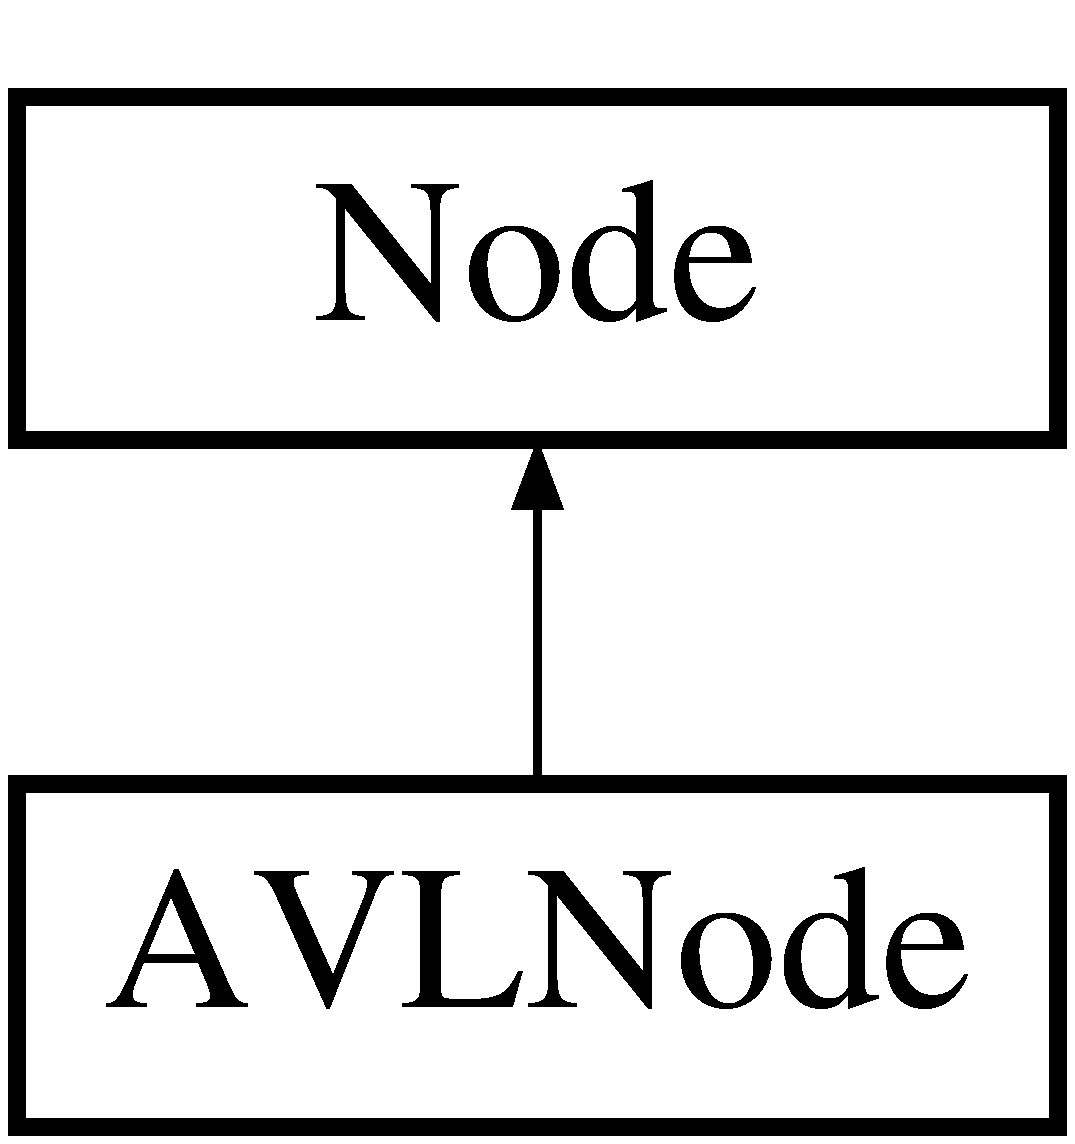
\includegraphics[height=2.000000cm]{class_a_v_l_node}
\end{center}
\end{figure}
\subsection*{Public Member Functions}
\begin{DoxyCompactItemize}
\item 
\hyperlink{class_a_v_l_node_ab4a77945ebefb824cb3d21a0f9f3a514}{A\+V\+L\+Node} ()
\item 
\hyperlink{class_a_v_l_node_af27568a3d6ad4d83e651a0cc0f4057aa}{A\+V\+L\+Node} (string, \hyperlink{class_page}{Page} $\ast$)
\item 
\hyperlink{class_a_v_l_node_ac549cb5dbe98c28f5335ceaf0f602111}{A\+V\+L\+Node} (string, \hyperlink{class_a_v_l_node}{A\+V\+L\+Node} $\ast$\&, \hyperlink{class_a_v_l_node}{A\+V\+L\+Node} $\ast$\&, \hyperlink{class_page}{Page} $\ast$)
\item 
\hyperlink{class_a_v_l_node_a5b3f7cdff426ea2ac77da59399e6a386}{$\sim$\+A\+V\+L\+Node} ()
\end{DoxyCompactItemize}
\subsection*{Friends}
\begin{DoxyCompactItemize}
\item 
class \hyperlink{class_a_v_l_node_abb802889854b7d6aebdc6c5a9f751b0e}{A\+V\+L\+Tree}
\end{DoxyCompactItemize}


\subsection{Detailed Description}
A\+V\+L \hyperlink{class_node}{Node} header file Sam Hunter and Morgan Monzingo node built for A\+V\+L tree 

\subsection{Constructor \& Destructor Documentation}
\hypertarget{class_a_v_l_node_ab4a77945ebefb824cb3d21a0f9f3a514}{}\index{A\+V\+L\+Node@{A\+V\+L\+Node}!A\+V\+L\+Node@{A\+V\+L\+Node}}
\index{A\+V\+L\+Node@{A\+V\+L\+Node}!A\+V\+L\+Node@{A\+V\+L\+Node}}
\subsubsection[{A\+V\+L\+Node}]{\setlength{\rightskip}{0pt plus 5cm}A\+V\+L\+Node\+::\+A\+V\+L\+Node (
\begin{DoxyParamCaption}
{}
\end{DoxyParamCaption}
)}\label{class_a_v_l_node_ab4a77945ebefb824cb3d21a0f9f3a514}
\hypertarget{class_a_v_l_node_af27568a3d6ad4d83e651a0cc0f4057aa}{}\index{A\+V\+L\+Node@{A\+V\+L\+Node}!A\+V\+L\+Node@{A\+V\+L\+Node}}
\index{A\+V\+L\+Node@{A\+V\+L\+Node}!A\+V\+L\+Node@{A\+V\+L\+Node}}
\subsubsection[{A\+V\+L\+Node}]{\setlength{\rightskip}{0pt plus 5cm}A\+V\+L\+Node\+::\+A\+V\+L\+Node (
\begin{DoxyParamCaption}
\item[{string}]{kw, }
\item[{{\bf Page} $\ast$}]{pg}
\end{DoxyParamCaption}
)}\label{class_a_v_l_node_af27568a3d6ad4d83e651a0cc0f4057aa}
\hypertarget{class_a_v_l_node_ac549cb5dbe98c28f5335ceaf0f602111}{}\index{A\+V\+L\+Node@{A\+V\+L\+Node}!A\+V\+L\+Node@{A\+V\+L\+Node}}
\index{A\+V\+L\+Node@{A\+V\+L\+Node}!A\+V\+L\+Node@{A\+V\+L\+Node}}
\subsubsection[{A\+V\+L\+Node}]{\setlength{\rightskip}{0pt plus 5cm}A\+V\+L\+Node\+::\+A\+V\+L\+Node (
\begin{DoxyParamCaption}
\item[{string}]{kw, }
\item[{{\bf A\+V\+L\+Node} $\ast$\&}]{rightnode, }
\item[{{\bf A\+V\+L\+Node} $\ast$\&}]{leftnode, }
\item[{{\bf Page} $\ast$}]{pg}
\end{DoxyParamCaption}
)}\label{class_a_v_l_node_ac549cb5dbe98c28f5335ceaf0f602111}
\hypertarget{class_a_v_l_node_a5b3f7cdff426ea2ac77da59399e6a386}{}\index{A\+V\+L\+Node@{A\+V\+L\+Node}!````~A\+V\+L\+Node@{$\sim$\+A\+V\+L\+Node}}
\index{````~A\+V\+L\+Node@{$\sim$\+A\+V\+L\+Node}!A\+V\+L\+Node@{A\+V\+L\+Node}}
\subsubsection[{$\sim$\+A\+V\+L\+Node}]{\setlength{\rightskip}{0pt plus 5cm}A\+V\+L\+Node\+::$\sim$\+A\+V\+L\+Node (
\begin{DoxyParamCaption}
{}
\end{DoxyParamCaption}
)}\label{class_a_v_l_node_a5b3f7cdff426ea2ac77da59399e6a386}


\subsection{Friends And Related Function Documentation}
\hypertarget{class_a_v_l_node_abb802889854b7d6aebdc6c5a9f751b0e}{}\index{A\+V\+L\+Node@{A\+V\+L\+Node}!A\+V\+L\+Tree@{A\+V\+L\+Tree}}
\index{A\+V\+L\+Tree@{A\+V\+L\+Tree}!A\+V\+L\+Node@{A\+V\+L\+Node}}
\subsubsection[{A\+V\+L\+Tree}]{\setlength{\rightskip}{0pt plus 5cm}friend class {\bf A\+V\+L\+Tree}\hspace{0.3cm}{\ttfamily [friend]}}\label{class_a_v_l_node_abb802889854b7d6aebdc6c5a9f751b0e}


The documentation for this class was generated from the following files\+:\begin{DoxyCompactItemize}
\item 
\hyperlink{_a_v_l_node_8h}{A\+V\+L\+Node.\+h}\item 
\hyperlink{_a_v_l_node_8cpp}{A\+V\+L\+Node.\+cpp}\end{DoxyCompactItemize}

\hypertarget{class_a_v_l_tree}{}\section{A\+V\+L\+Tree Class Reference}
\label{class_a_v_l_tree}\index{A\+V\+L\+Tree@{A\+V\+L\+Tree}}


{\ttfamily \#include $<$A\+V\+L\+Tree.\+h$>$}

Inheritance diagram for A\+V\+L\+Tree\+:\begin{figure}[H]
\begin{center}
\leavevmode
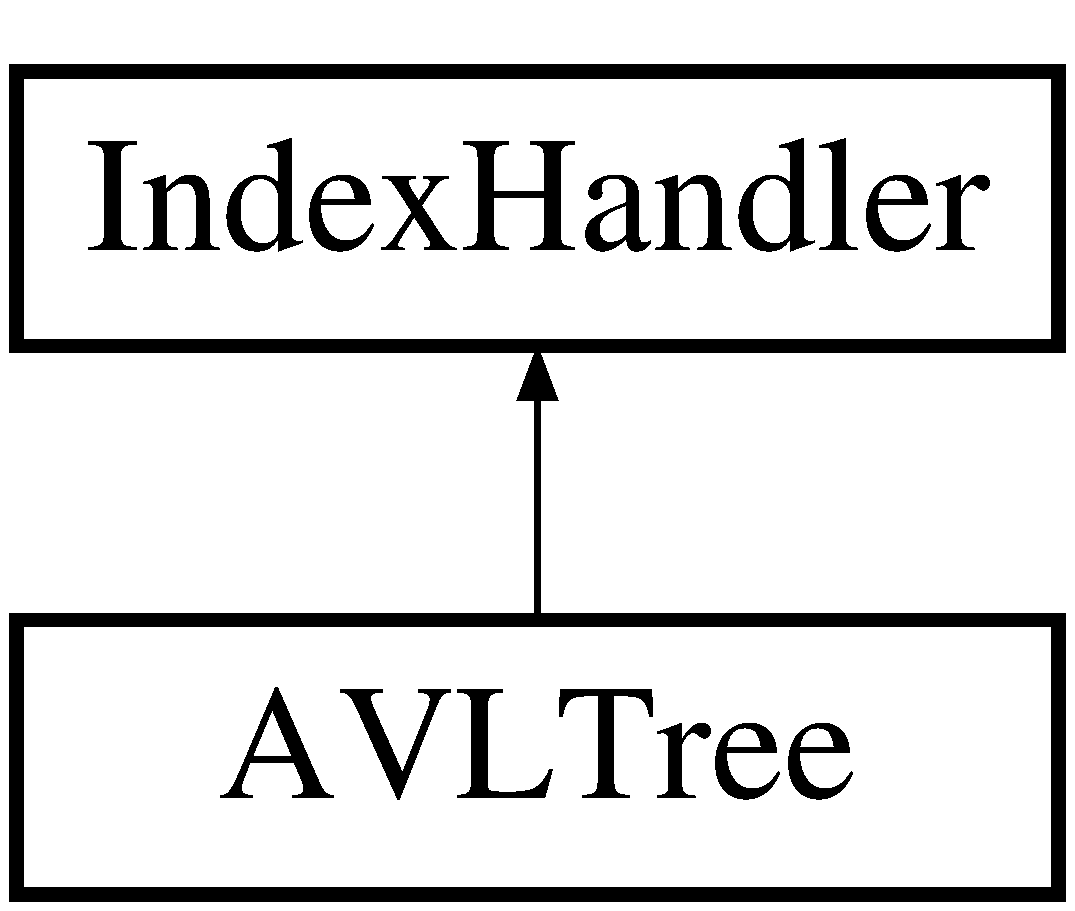
\includegraphics[height=2.000000cm]{class_a_v_l_tree}
\end{center}
\end{figure}
\subsection*{Public Member Functions}
\begin{DoxyCompactItemize}
\item 
\hyperlink{class_a_v_l_tree_a0915d328ebed07e11087692f17d80827}{A\+V\+L\+Tree} ()
\item 
\hyperlink{class_a_v_l_tree_af4a1d1be1b6301ba59c6e101c6efc6ba}{$\sim$\+A\+V\+L\+Tree} ()
\item 
void \hyperlink{class_a_v_l_tree_acc05c3c67a02da11ae973a01c37ae89e}{add\+To\+Index} (\hyperlink{class_page}{Page} $\ast$\&, string \&)
\item 
\hyperlink{class_a_v_l_node}{A\+V\+L\+Node} $\ast$\& \hyperlink{class_a_v_l_tree_a0e9a469764ef2056ffc1257ace172612}{insert} (string \&, \hyperlink{class_page}{Page} $\ast$\&, \hyperlink{class_a_v_l_node}{A\+V\+L\+Node} $\ast$\&)
\item 
\hyperlink{class_a_v_l_node}{A\+V\+L\+Node} $\ast$\& \hyperlink{class_a_v_l_tree_a6f77603032cfc0477eae2fc8944cec75}{balance} (\hyperlink{class_a_v_l_node}{A\+V\+L\+Node} $\ast$)
\item 
set$<$ \hyperlink{class_page}{Page} $\ast$ $>$ \hyperlink{class_a_v_l_tree_a7b6bc9d63cff082843ac1de050268f2d}{search\+Index} (string)
\item 
set$<$ \hyperlink{class_page}{Page} $\ast$ $>$ \hyperlink{class_a_v_l_tree_ac439d90d1a41fc1526e5882ba25f2a5b}{search} (string, \hyperlink{class_a_v_l_node}{A\+V\+L\+Node} $\ast$\&)
\item 
int \hyperlink{class_a_v_l_tree_ad3fb38e4b3f05d203dbc1d5c87be48b0}{height} (\hyperlink{class_a_v_l_node}{A\+V\+L\+Node} $\ast$)
\item 
int \hyperlink{class_a_v_l_tree_a4ba40b6b969fe541c840ac2e3ad1dd48}{difference} (\hyperlink{class_a_v_l_node}{A\+V\+L\+Node} $\ast$)
\item 
\hyperlink{class_a_v_l_node}{A\+V\+L\+Node} $\ast$\& \hyperlink{class_a_v_l_tree_ac861efd40852530f890f75af8adb05d3}{left\+Rotation} (\hyperlink{class_a_v_l_node}{A\+V\+L\+Node} $\ast$)
\begin{DoxyCompactList}\small\item\em rotations \end{DoxyCompactList}\item 
\hyperlink{class_a_v_l_node}{A\+V\+L\+Node} $\ast$\& \hyperlink{class_a_v_l_tree_a3d119fc1729d30c627b125f01dfa713f}{right\+Rotation} (\hyperlink{class_a_v_l_node}{A\+V\+L\+Node} $\ast$)
\item 
\hyperlink{class_a_v_l_node}{A\+V\+L\+Node} $\ast$\& \hyperlink{class_a_v_l_tree_aae25b3c2ba45785f14e6460f7da27a90}{double\+Left} (\hyperlink{class_a_v_l_node}{A\+V\+L\+Node} $\ast$)
\item 
\hyperlink{class_a_v_l_node}{A\+V\+L\+Node} $\ast$\& \hyperlink{class_a_v_l_tree_a52414545fb12fa95fd4b48410e32a90f}{double\+Right} (\hyperlink{class_a_v_l_node}{A\+V\+L\+Node} $\ast$)
\item 
void \hyperlink{class_a_v_l_tree_aaeb00045be61c381863d43526b4dffe1}{print\+Table} ()
\item 
void \hyperlink{class_a_v_l_tree_aadb95e92d5560738574ae428ae2df980}{display} (\hyperlink{class_a_v_l_node}{A\+V\+L\+Node} $\ast$, int)
\item 
void \hyperlink{class_a_v_l_tree_a3857ebba2ac14e0fd1ded8f1c6cb224c}{inorder} (\hyperlink{class_a_v_l_node}{A\+V\+L\+Node} $\ast$)
\item 
string \hyperlink{class_a_v_l_tree_a708b6398ea1771de3077ca39c4005cca}{get\+Class\+Type} ()
\end{DoxyCompactItemize}
\subsection*{Friends}
\begin{DoxyCompactItemize}
\item 
class \hyperlink{class_a_v_l_tree_aefbabd2f704298b266a25d1a555a63f0}{A\+V\+L\+Node}
\end{DoxyCompactItemize}


\subsection{Constructor \& Destructor Documentation}
\hypertarget{class_a_v_l_tree_a0915d328ebed07e11087692f17d80827}{}\index{A\+V\+L\+Tree@{A\+V\+L\+Tree}!A\+V\+L\+Tree@{A\+V\+L\+Tree}}
\index{A\+V\+L\+Tree@{A\+V\+L\+Tree}!A\+V\+L\+Tree@{A\+V\+L\+Tree}}
\subsubsection[{A\+V\+L\+Tree}]{\setlength{\rightskip}{0pt plus 5cm}A\+V\+L\+Tree\+::\+A\+V\+L\+Tree (
\begin{DoxyParamCaption}
{}
\end{DoxyParamCaption}
)}\label{class_a_v_l_tree_a0915d328ebed07e11087692f17d80827}
\hypertarget{class_a_v_l_tree_af4a1d1be1b6301ba59c6e101c6efc6ba}{}\index{A\+V\+L\+Tree@{A\+V\+L\+Tree}!````~A\+V\+L\+Tree@{$\sim$\+A\+V\+L\+Tree}}
\index{````~A\+V\+L\+Tree@{$\sim$\+A\+V\+L\+Tree}!A\+V\+L\+Tree@{A\+V\+L\+Tree}}
\subsubsection[{$\sim$\+A\+V\+L\+Tree}]{\setlength{\rightskip}{0pt plus 5cm}A\+V\+L\+Tree\+::$\sim$\+A\+V\+L\+Tree (
\begin{DoxyParamCaption}
{}
\end{DoxyParamCaption}
)}\label{class_a_v_l_tree_af4a1d1be1b6301ba59c6e101c6efc6ba}


\subsection{Member Function Documentation}
\hypertarget{class_a_v_l_tree_acc05c3c67a02da11ae973a01c37ae89e}{}\index{A\+V\+L\+Tree@{A\+V\+L\+Tree}!add\+To\+Index@{add\+To\+Index}}
\index{add\+To\+Index@{add\+To\+Index}!A\+V\+L\+Tree@{A\+V\+L\+Tree}}
\subsubsection[{add\+To\+Index}]{\setlength{\rightskip}{0pt plus 5cm}void A\+V\+L\+Tree\+::add\+To\+Index (
\begin{DoxyParamCaption}
\item[{{\bf Page} $\ast$\&}]{pg, }
\item[{string \&}]{kw}
\end{DoxyParamCaption}
)}\label{class_a_v_l_tree_acc05c3c67a02da11ae973a01c37ae89e}
\hypertarget{class_a_v_l_tree_a6f77603032cfc0477eae2fc8944cec75}{}\index{A\+V\+L\+Tree@{A\+V\+L\+Tree}!balance@{balance}}
\index{balance@{balance}!A\+V\+L\+Tree@{A\+V\+L\+Tree}}
\subsubsection[{balance}]{\setlength{\rightskip}{0pt plus 5cm}{\bf A\+V\+L\+Node} $\ast$\& A\+V\+L\+Tree\+::balance (
\begin{DoxyParamCaption}
\item[{{\bf A\+V\+L\+Node} $\ast$}]{avlnode}
\end{DoxyParamCaption}
)}\label{class_a_v_l_tree_a6f77603032cfc0477eae2fc8944cec75}
\hypertarget{class_a_v_l_tree_a4ba40b6b969fe541c840ac2e3ad1dd48}{}\index{A\+V\+L\+Tree@{A\+V\+L\+Tree}!difference@{difference}}
\index{difference@{difference}!A\+V\+L\+Tree@{A\+V\+L\+Tree}}
\subsubsection[{difference}]{\setlength{\rightskip}{0pt plus 5cm}int A\+V\+L\+Tree\+::difference (
\begin{DoxyParamCaption}
\item[{{\bf A\+V\+L\+Node} $\ast$}]{avlnode}
\end{DoxyParamCaption}
)}\label{class_a_v_l_tree_a4ba40b6b969fe541c840ac2e3ad1dd48}
\hypertarget{class_a_v_l_tree_aadb95e92d5560738574ae428ae2df980}{}\index{A\+V\+L\+Tree@{A\+V\+L\+Tree}!display@{display}}
\index{display@{display}!A\+V\+L\+Tree@{A\+V\+L\+Tree}}
\subsubsection[{display}]{\setlength{\rightskip}{0pt plus 5cm}void A\+V\+L\+Tree\+::display (
\begin{DoxyParamCaption}
\item[{{\bf A\+V\+L\+Node} $\ast$}]{ptr, }
\item[{int}]{level}
\end{DoxyParamCaption}
)}\label{class_a_v_l_tree_aadb95e92d5560738574ae428ae2df980}
\hypertarget{class_a_v_l_tree_aae25b3c2ba45785f14e6460f7da27a90}{}\index{A\+V\+L\+Tree@{A\+V\+L\+Tree}!double\+Left@{double\+Left}}
\index{double\+Left@{double\+Left}!A\+V\+L\+Tree@{A\+V\+L\+Tree}}
\subsubsection[{double\+Left}]{\setlength{\rightskip}{0pt plus 5cm}{\bf A\+V\+L\+Node} $\ast$\& A\+V\+L\+Tree\+::double\+Left (
\begin{DoxyParamCaption}
\item[{{\bf A\+V\+L\+Node} $\ast$}]{avlnode}
\end{DoxyParamCaption}
)}\label{class_a_v_l_tree_aae25b3c2ba45785f14e6460f7da27a90}
\hypertarget{class_a_v_l_tree_a52414545fb12fa95fd4b48410e32a90f}{}\index{A\+V\+L\+Tree@{A\+V\+L\+Tree}!double\+Right@{double\+Right}}
\index{double\+Right@{double\+Right}!A\+V\+L\+Tree@{A\+V\+L\+Tree}}
\subsubsection[{double\+Right}]{\setlength{\rightskip}{0pt plus 5cm}{\bf A\+V\+L\+Node} $\ast$\& A\+V\+L\+Tree\+::double\+Right (
\begin{DoxyParamCaption}
\item[{{\bf A\+V\+L\+Node} $\ast$}]{avlnode}
\end{DoxyParamCaption}
)}\label{class_a_v_l_tree_a52414545fb12fa95fd4b48410e32a90f}
\hypertarget{class_a_v_l_tree_a708b6398ea1771de3077ca39c4005cca}{}\index{A\+V\+L\+Tree@{A\+V\+L\+Tree}!get\+Class\+Type@{get\+Class\+Type}}
\index{get\+Class\+Type@{get\+Class\+Type}!A\+V\+L\+Tree@{A\+V\+L\+Tree}}
\subsubsection[{get\+Class\+Type}]{\setlength{\rightskip}{0pt plus 5cm}string A\+V\+L\+Tree\+::get\+Class\+Type (
\begin{DoxyParamCaption}
{}
\end{DoxyParamCaption}
)\hspace{0.3cm}{\ttfamily [virtual]}}\label{class_a_v_l_tree_a708b6398ea1771de3077ca39c4005cca}


Implements \hyperlink{class_index_handler_aaeb0f250516fbc93936efec2c3f21359}{Index\+Handler}.

\hypertarget{class_a_v_l_tree_ad3fb38e4b3f05d203dbc1d5c87be48b0}{}\index{A\+V\+L\+Tree@{A\+V\+L\+Tree}!height@{height}}
\index{height@{height}!A\+V\+L\+Tree@{A\+V\+L\+Tree}}
\subsubsection[{height}]{\setlength{\rightskip}{0pt plus 5cm}int A\+V\+L\+Tree\+::height (
\begin{DoxyParamCaption}
\item[{{\bf A\+V\+L\+Node} $\ast$}]{avlnode}
\end{DoxyParamCaption}
)}\label{class_a_v_l_tree_ad3fb38e4b3f05d203dbc1d5c87be48b0}
\hypertarget{class_a_v_l_tree_a3857ebba2ac14e0fd1ded8f1c6cb224c}{}\index{A\+V\+L\+Tree@{A\+V\+L\+Tree}!inorder@{inorder}}
\index{inorder@{inorder}!A\+V\+L\+Tree@{A\+V\+L\+Tree}}
\subsubsection[{inorder}]{\setlength{\rightskip}{0pt plus 5cm}void A\+V\+L\+Tree\+::inorder (
\begin{DoxyParamCaption}
\item[{{\bf A\+V\+L\+Node} $\ast$}]{temp}
\end{DoxyParamCaption}
)}\label{class_a_v_l_tree_a3857ebba2ac14e0fd1ded8f1c6cb224c}
\hypertarget{class_a_v_l_tree_a0e9a469764ef2056ffc1257ace172612}{}\index{A\+V\+L\+Tree@{A\+V\+L\+Tree}!insert@{insert}}
\index{insert@{insert}!A\+V\+L\+Tree@{A\+V\+L\+Tree}}
\subsubsection[{insert}]{\setlength{\rightskip}{0pt plus 5cm}{\bf A\+V\+L\+Node} $\ast$\& A\+V\+L\+Tree\+::insert (
\begin{DoxyParamCaption}
\item[{string \&}]{kw, }
\item[{{\bf Page} $\ast$\&}]{pg, }
\item[{{\bf A\+V\+L\+Node} $\ast$\&}]{avlnode}
\end{DoxyParamCaption}
)}\label{class_a_v_l_tree_a0e9a469764ef2056ffc1257ace172612}
\hypertarget{class_a_v_l_tree_ac861efd40852530f890f75af8adb05d3}{}\index{A\+V\+L\+Tree@{A\+V\+L\+Tree}!left\+Rotation@{left\+Rotation}}
\index{left\+Rotation@{left\+Rotation}!A\+V\+L\+Tree@{A\+V\+L\+Tree}}
\subsubsection[{left\+Rotation}]{\setlength{\rightskip}{0pt plus 5cm}{\bf A\+V\+L\+Node} $\ast$\& A\+V\+L\+Tree\+::left\+Rotation (
\begin{DoxyParamCaption}
\item[{{\bf A\+V\+L\+Node} $\ast$}]{avlnode}
\end{DoxyParamCaption}
)}\label{class_a_v_l_tree_ac861efd40852530f890f75af8adb05d3}


rotations 

\hypertarget{class_a_v_l_tree_aaeb00045be61c381863d43526b4dffe1}{}\index{A\+V\+L\+Tree@{A\+V\+L\+Tree}!print\+Table@{print\+Table}}
\index{print\+Table@{print\+Table}!A\+V\+L\+Tree@{A\+V\+L\+Tree}}
\subsubsection[{print\+Table}]{\setlength{\rightskip}{0pt plus 5cm}void A\+V\+L\+Tree\+::print\+Table (
\begin{DoxyParamCaption}
{}
\end{DoxyParamCaption}
)\hspace{0.3cm}{\ttfamily [virtual]}}\label{class_a_v_l_tree_aaeb00045be61c381863d43526b4dffe1}


Implements \hyperlink{class_index_handler_a036ccca02cb734711a1e6a50b09a2b1f}{Index\+Handler}.

\hypertarget{class_a_v_l_tree_a3d119fc1729d30c627b125f01dfa713f}{}\index{A\+V\+L\+Tree@{A\+V\+L\+Tree}!right\+Rotation@{right\+Rotation}}
\index{right\+Rotation@{right\+Rotation}!A\+V\+L\+Tree@{A\+V\+L\+Tree}}
\subsubsection[{right\+Rotation}]{\setlength{\rightskip}{0pt plus 5cm}{\bf A\+V\+L\+Node} $\ast$\& A\+V\+L\+Tree\+::right\+Rotation (
\begin{DoxyParamCaption}
\item[{{\bf A\+V\+L\+Node} $\ast$}]{avlnode}
\end{DoxyParamCaption}
)}\label{class_a_v_l_tree_a3d119fc1729d30c627b125f01dfa713f}
\hypertarget{class_a_v_l_tree_ac439d90d1a41fc1526e5882ba25f2a5b}{}\index{A\+V\+L\+Tree@{A\+V\+L\+Tree}!search@{search}}
\index{search@{search}!A\+V\+L\+Tree@{A\+V\+L\+Tree}}
\subsubsection[{search}]{\setlength{\rightskip}{0pt plus 5cm}set$<$ {\bf Page} $\ast$ $>$ A\+V\+L\+Tree\+::search (
\begin{DoxyParamCaption}
\item[{string}]{search\+\_\+string, }
\item[{{\bf A\+V\+L\+Node} $\ast$\&}]{root}
\end{DoxyParamCaption}
)}\label{class_a_v_l_tree_ac439d90d1a41fc1526e5882ba25f2a5b}
\hypertarget{class_a_v_l_tree_a7b6bc9d63cff082843ac1de050268f2d}{}\index{A\+V\+L\+Tree@{A\+V\+L\+Tree}!search\+Index@{search\+Index}}
\index{search\+Index@{search\+Index}!A\+V\+L\+Tree@{A\+V\+L\+Tree}}
\subsubsection[{search\+Index}]{\setlength{\rightskip}{0pt plus 5cm}set$<$ {\bf Page} $\ast$ $>$ A\+V\+L\+Tree\+::search\+Index (
\begin{DoxyParamCaption}
\item[{string}]{search\+\_\+term}
\end{DoxyParamCaption}
)}\label{class_a_v_l_tree_a7b6bc9d63cff082843ac1de050268f2d}


\subsection{Friends And Related Function Documentation}
\hypertarget{class_a_v_l_tree_aefbabd2f704298b266a25d1a555a63f0}{}\index{A\+V\+L\+Tree@{A\+V\+L\+Tree}!A\+V\+L\+Node@{A\+V\+L\+Node}}
\index{A\+V\+L\+Node@{A\+V\+L\+Node}!A\+V\+L\+Tree@{A\+V\+L\+Tree}}
\subsubsection[{A\+V\+L\+Node}]{\setlength{\rightskip}{0pt plus 5cm}friend class {\bf A\+V\+L\+Node}\hspace{0.3cm}{\ttfamily [friend]}}\label{class_a_v_l_tree_aefbabd2f704298b266a25d1a555a63f0}


The documentation for this class was generated from the following files\+:\begin{DoxyCompactItemize}
\item 
\hyperlink{_a_v_l_tree_8h}{A\+V\+L\+Tree.\+h}\item 
\hyperlink{_a_v_l_tree_8cpp}{A\+V\+L\+Tree.\+cpp}\end{DoxyCompactItemize}

\hypertarget{class_document_parser}{\section{Document\+Parser Class Reference}
\label{class_document_parser}\index{Document\+Parser@{Document\+Parser}}
}
\subsection*{Public Member Functions}
\begin{DoxyCompactItemize}
\item 
\hypertarget{class_document_parser_a40fc3f32cbe2d6f4f978caa42ee509d6}{void {\bfseries parse\+Drive} (string, \hyperlink{class_index_handler}{Index\+Handler} $\ast$\&)}\label{class_document_parser_a40fc3f32cbe2d6f4f978caa42ee509d6}

\item 
\hypertarget{class_document_parser_ae132955b8118c74df2705defd1fe856b}{void {\bfseries send\+To\+Index} (\hyperlink{class_page}{Page} $\ast$)}\label{class_document_parser_ae132955b8118c74df2705defd1fe856b}

\item 
\hypertarget{class_document_parser_a7ca97302ad273efde7f33163ab9e78dc}{void {\bfseries write\+To\+Structure} (\hyperlink{class_index_handler}{Index\+Handler} $\ast$\&, int start\+Index=0)}\label{class_document_parser_a7ca97302ad273efde7f33163ab9e78dc}

\item 
\hypertarget{class_document_parser_a8f07107cbe76401f9db73dbf9cae7a5f}{void {\bfseries save\+Index} ()}\label{class_document_parser_a8f07107cbe76401f9db73dbf9cae7a5f}

\item 
\hypertarget{class_document_parser_a8046232e6026fb59d3052426e7ed7a58}{void {\bfseries read\+In\+Parsed\+File} (\hyperlink{class_index_handler}{Index\+Handler} $\ast$\&)}\label{class_document_parser_a8046232e6026fb59d3052426e7ed7a58}

\item 
\hypertarget{class_document_parser_a23dd86d1fb040662e97845d2499e5ae1}{int {\bfseries get\+Collection\+Size} ()}\label{class_document_parser_a23dd86d1fb040662e97845d2499e5ae1}

\end{DoxyCompactItemize}


The documentation for this class was generated from the following files\+:\begin{DoxyCompactItemize}
\item 
Document\+Parser.\+h\item 
Document\+Parser.\+cpp\end{DoxyCompactItemize}

\hypertarget{class_hash_node}{\section{Hash\+Node Class Reference}
\label{class_hash_node}\index{Hash\+Node@{Hash\+Node}}
}
Inheritance diagram for Hash\+Node\+:\begin{figure}[H]
\begin{center}
\leavevmode
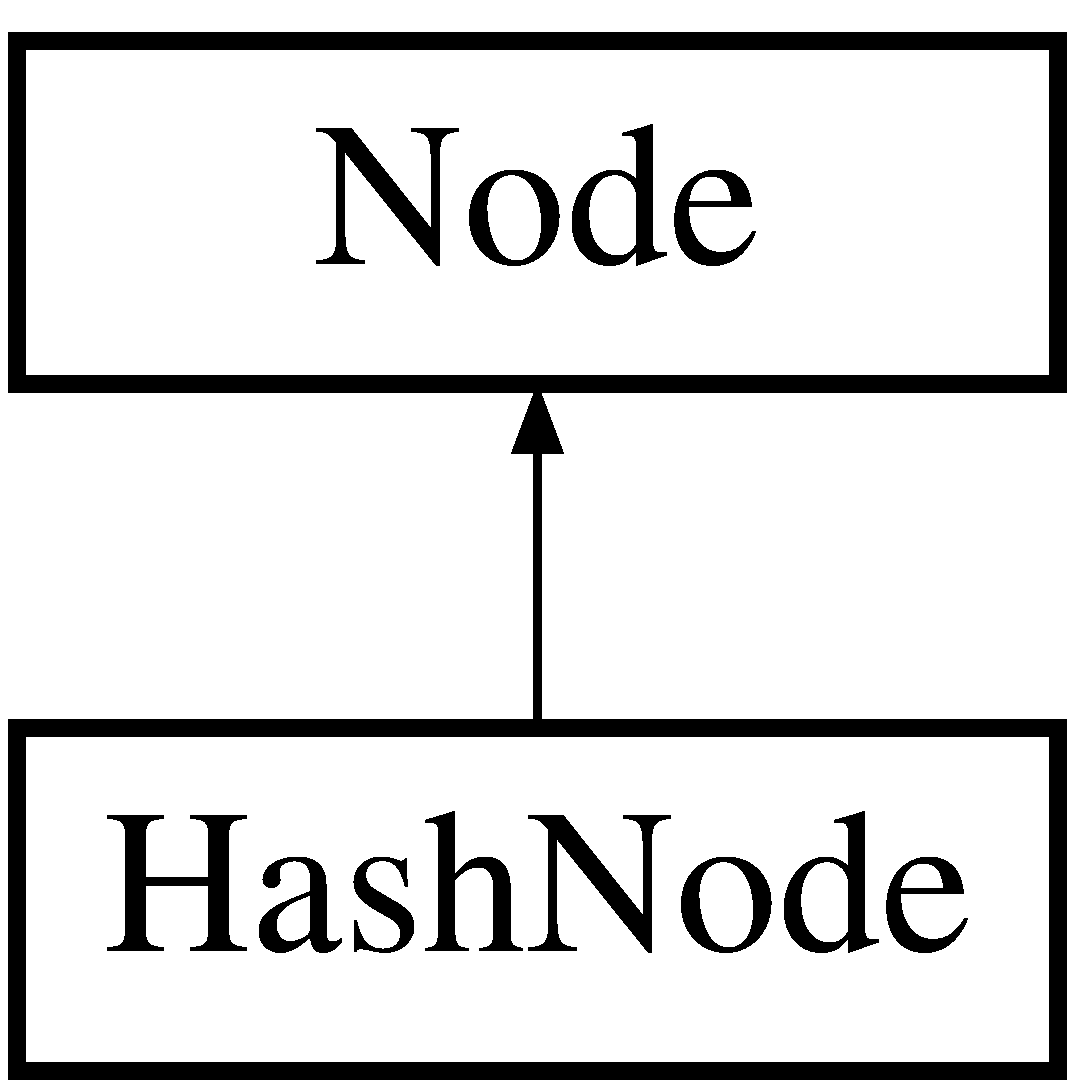
\includegraphics[height=2.000000cm]{class_hash_node}
\end{center}
\end{figure}
\subsection*{Public Member Functions}
\begin{DoxyCompactItemize}
\item 
\hypertarget{class_hash_node_af85be330cc34bb55f26041c7224b5b25}{{\bfseries Hash\+Node} (\hyperlink{class_node}{Node} $\ast$\&other)}\label{class_hash_node_af85be330cc34bb55f26041c7224b5b25}

\item 
\hypertarget{class_hash_node_ae3a3c1f03c060e03cc01ef81aae2c734}{\hyperlink{class_hash_node}{Hash\+Node} $\ast$ {\bfseries get\+Next\+Hash\+Node} ()}\label{class_hash_node_ae3a3c1f03c060e03cc01ef81aae2c734}

\item 
\hypertarget{class_hash_node_a0711b28c4cbdb8a21e6df486896081b3}{void {\bfseries set\+Next\+Hash\+Node} (\hyperlink{class_hash_node}{Hash\+Node} $\ast$)}\label{class_hash_node_a0711b28c4cbdb8a21e6df486896081b3}

\end{DoxyCompactItemize}
\subsection*{Friends}
\begin{DoxyCompactItemize}
\item 
\hypertarget{class_hash_node_a574ea806a7ec4e2f0fa54ed7da67b628}{class {\bfseries Hash\+Table}}\label{class_hash_node_a574ea806a7ec4e2f0fa54ed7da67b628}

\end{DoxyCompactItemize}


The documentation for this class was generated from the following files\+:\begin{DoxyCompactItemize}
\item 
Hash\+Node.\+h\item 
Hash\+Node.\+cpp\end{DoxyCompactItemize}

\hypertarget{class_hash_table}{\section{Hash\+Table Class Reference}
\label{class_hash_table}\index{Hash\+Table@{Hash\+Table}}
}
Inheritance diagram for Hash\+Table\+:\begin{figure}[H]
\begin{center}
\leavevmode
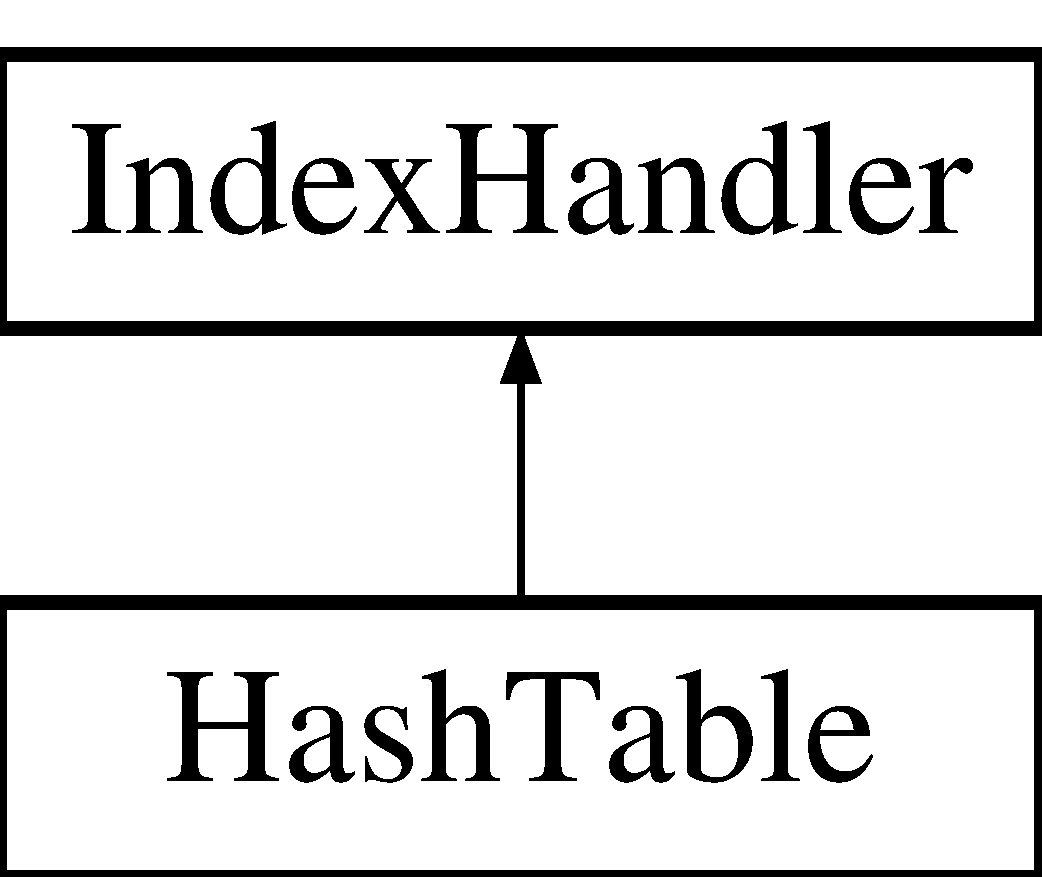
\includegraphics[height=2.000000cm]{class_hash_table}
\end{center}
\end{figure}
\subsection*{Public Member Functions}
\begin{DoxyCompactItemize}
\item 
\hypertarget{class_hash_table_aaa6417f06baad4f297d098dc7393e48b}{void {\bfseries add\+To\+Index} (\hyperlink{class_page}{Page} $\ast$\&, string \&)}\label{class_hash_table_aaa6417f06baad4f297d098dc7393e48b}

\item 
\hypertarget{class_hash_table_ab50be186df67a5621694cb2f692de3fa}{void {\bfseries print\+Table} ()}\label{class_hash_table_ab50be186df67a5621694cb2f692de3fa}

\item 
\hypertarget{class_hash_table_a838109ea89fa1b80908aee6838d96ad1}{set$<$ \hyperlink{class_page}{Page} $\ast$ $>$ {\bfseries search\+Index} (string)}\label{class_hash_table_a838109ea89fa1b80908aee6838d96ad1}

\item 
\hypertarget{class_hash_table_ad42a8eb156c387de2645ca1276ea412a}{void {\bfseries save\+Index} ()}\label{class_hash_table_ad42a8eb156c387de2645ca1276ea412a}

\item 
\hypertarget{class_hash_table_ab5a5fca28242a0733cb95e0729d94761}{string {\bfseries get\+Class\+Type} ()}\label{class_hash_table_ab5a5fca28242a0733cb95e0729d94761}

\item 
\hypertarget{class_hash_table_acf96b4d4e320ab83fbeed1578a415be8}{void {\bfseries destroy\+Structure} ()}\label{class_hash_table_acf96b4d4e320ab83fbeed1578a415be8}

\end{DoxyCompactItemize}


The documentation for this class was generated from the following files\+:\begin{DoxyCompactItemize}
\item 
Hash\+Table.\+h\item 
Hash\+Table.\+cpp\end{DoxyCompactItemize}

\hypertarget{class_index_handler}{}\section{Index\+Handler Class Reference}
\label{class_index_handler}\index{Index\+Handler@{Index\+Handler}}


{\ttfamily \#include $<$Index\+Handler.\+h$>$}

Inheritance diagram for Index\+Handler\+:\begin{figure}[H]
\begin{center}
\leavevmode
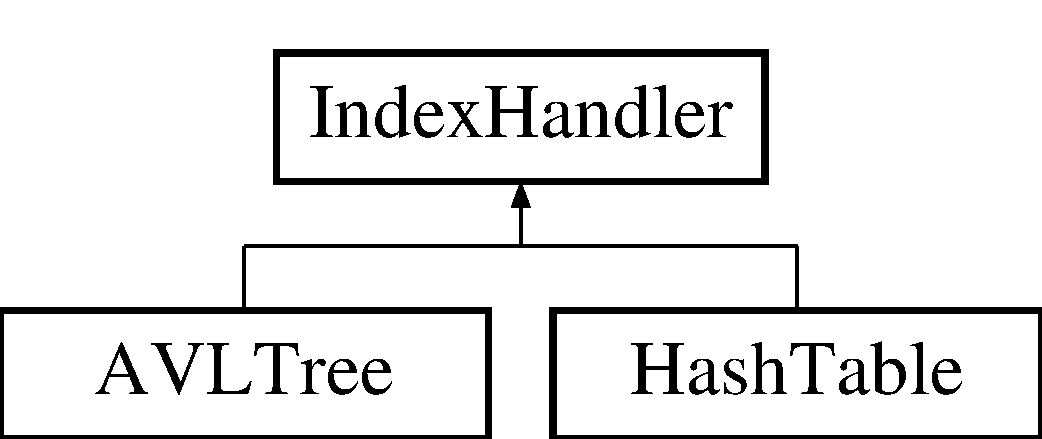
\includegraphics[height=2.000000cm]{class_index_handler}
\end{center}
\end{figure}
\subsection*{Public Member Functions}
\begin{DoxyCompactItemize}
\item 
\hyperlink{class_index_handler_a27748387661142a2eb545be6f0499996}{Index\+Handler} ()
\item 
virtual \hyperlink{class_index_handler_ad787ca8cf83345ecfe332d2c3b8f8009}{$\sim$\+Index\+Handler} ()
\item 
virtual std\+::string \hyperlink{class_index_handler_aaeb0f250516fbc93936efec2c3f21359}{get\+Class\+Type} ()=0
\item 
void \hyperlink{class_index_handler_aa916a3613990ed790d281863d685cfc5}{add\+Page} (\hyperlink{class_page}{Page} $\ast$)
\item 
virtual void \hyperlink{class_index_handler_a102638a9813e71541092a6695bd24012}{add\+To\+Index} (\hyperlink{class_page}{Page} $\ast$\&, std\+::string \&)=0
\item 
virtual set$<$ \hyperlink{class_page}{Page} $\ast$ $>$ \hyperlink{class_index_handler_ac3213de7636a1332440c3204957f4658}{search\+Index} (std\+::string)=0
\item 
virtual void \hyperlink{class_index_handler_a036ccca02cb734711a1e6a50b09a2b1f}{print\+Table} ()=0
\end{DoxyCompactItemize}


\subsection{Constructor \& Destructor Documentation}
\hypertarget{class_index_handler_a27748387661142a2eb545be6f0499996}{}\index{Index\+Handler@{Index\+Handler}!Index\+Handler@{Index\+Handler}}
\index{Index\+Handler@{Index\+Handler}!Index\+Handler@{Index\+Handler}}
\subsubsection[{Index\+Handler}]{\setlength{\rightskip}{0pt plus 5cm}Index\+Handler\+::\+Index\+Handler (
\begin{DoxyParamCaption}
{}
\end{DoxyParamCaption}
)}\label{class_index_handler_a27748387661142a2eb545be6f0499996}
\hypertarget{class_index_handler_ad787ca8cf83345ecfe332d2c3b8f8009}{}\index{Index\+Handler@{Index\+Handler}!````~Index\+Handler@{$\sim$\+Index\+Handler}}
\index{````~Index\+Handler@{$\sim$\+Index\+Handler}!Index\+Handler@{Index\+Handler}}
\subsubsection[{$\sim$\+Index\+Handler}]{\setlength{\rightskip}{0pt plus 5cm}Index\+Handler\+::$\sim$\+Index\+Handler (
\begin{DoxyParamCaption}
{}
\end{DoxyParamCaption}
)\hspace{0.3cm}{\ttfamily [virtual]}}\label{class_index_handler_ad787ca8cf83345ecfe332d2c3b8f8009}


\subsection{Member Function Documentation}
\hypertarget{class_index_handler_aa916a3613990ed790d281863d685cfc5}{}\index{Index\+Handler@{Index\+Handler}!add\+Page@{add\+Page}}
\index{add\+Page@{add\+Page}!Index\+Handler@{Index\+Handler}}
\subsubsection[{add\+Page}]{\setlength{\rightskip}{0pt plus 5cm}void Index\+Handler\+::add\+Page (
\begin{DoxyParamCaption}
\item[{{\bf Page} $\ast$}]{next\+Page}
\end{DoxyParamCaption}
)}\label{class_index_handler_aa916a3613990ed790d281863d685cfc5}
\hypertarget{class_index_handler_a102638a9813e71541092a6695bd24012}{}\index{Index\+Handler@{Index\+Handler}!add\+To\+Index@{add\+To\+Index}}
\index{add\+To\+Index@{add\+To\+Index}!Index\+Handler@{Index\+Handler}}
\subsubsection[{add\+To\+Index}]{\setlength{\rightskip}{0pt plus 5cm}virtual void Index\+Handler\+::add\+To\+Index (
\begin{DoxyParamCaption}
\item[{{\bf Page} $\ast$\&}]{, }
\item[{std\+::string \&}]{}
\end{DoxyParamCaption}
)\hspace{0.3cm}{\ttfamily [pure virtual]}}\label{class_index_handler_a102638a9813e71541092a6695bd24012}


Implemented in \hyperlink{class_hash_table_a9bee171516cca4930348a89fd0695b08}{Hash\+Table}.

\hypertarget{class_index_handler_aaeb0f250516fbc93936efec2c3f21359}{}\index{Index\+Handler@{Index\+Handler}!get\+Class\+Type@{get\+Class\+Type}}
\index{get\+Class\+Type@{get\+Class\+Type}!Index\+Handler@{Index\+Handler}}
\subsubsection[{get\+Class\+Type}]{\setlength{\rightskip}{0pt plus 5cm}virtual std\+::string Index\+Handler\+::get\+Class\+Type (
\begin{DoxyParamCaption}
{}
\end{DoxyParamCaption}
)\hspace{0.3cm}{\ttfamily [pure virtual]}}\label{class_index_handler_aaeb0f250516fbc93936efec2c3f21359}


Implemented in \hyperlink{class_a_v_l_tree_a708b6398ea1771de3077ca39c4005cca}{A\+V\+L\+Tree}, and \hyperlink{class_hash_table_ab5a5fca28242a0733cb95e0729d94761}{Hash\+Table}.

\hypertarget{class_index_handler_a036ccca02cb734711a1e6a50b09a2b1f}{}\index{Index\+Handler@{Index\+Handler}!print\+Table@{print\+Table}}
\index{print\+Table@{print\+Table}!Index\+Handler@{Index\+Handler}}
\subsubsection[{print\+Table}]{\setlength{\rightskip}{0pt plus 5cm}virtual void Index\+Handler\+::print\+Table (
\begin{DoxyParamCaption}
{}
\end{DoxyParamCaption}
)\hspace{0.3cm}{\ttfamily [pure virtual]}}\label{class_index_handler_a036ccca02cb734711a1e6a50b09a2b1f}


Implemented in \hyperlink{class_a_v_l_tree_aaeb00045be61c381863d43526b4dffe1}{A\+V\+L\+Tree}, and \hyperlink{class_hash_table_ab50be186df67a5621694cb2f692de3fa}{Hash\+Table}.

\hypertarget{class_index_handler_ac3213de7636a1332440c3204957f4658}{}\index{Index\+Handler@{Index\+Handler}!search\+Index@{search\+Index}}
\index{search\+Index@{search\+Index}!Index\+Handler@{Index\+Handler}}
\subsubsection[{search\+Index}]{\setlength{\rightskip}{0pt plus 5cm}virtual set$<${\bf Page}$\ast$$>$ Index\+Handler\+::search\+Index (
\begin{DoxyParamCaption}
\item[{std\+::string}]{}
\end{DoxyParamCaption}
)\hspace{0.3cm}{\ttfamily [pure virtual]}}\label{class_index_handler_ac3213de7636a1332440c3204957f4658}


Implemented in \hyperlink{class_hash_table_a3e63955ddf861d2feb8e6db908c19ac9}{Hash\+Table}.



The documentation for this class was generated from the following files\+:\begin{DoxyCompactItemize}
\item 
\hyperlink{_index_handler_8h}{Index\+Handler.\+h}\item 
\hyperlink{_index_handler_8cpp}{Index\+Handler.\+cpp}\end{DoxyCompactItemize}

\hypertarget{class_node}{\section{Node Class Reference}
\label{class_node}\index{Node@{Node}}
}
Inheritance diagram for Node\+:\begin{figure}[H]
\begin{center}
\leavevmode
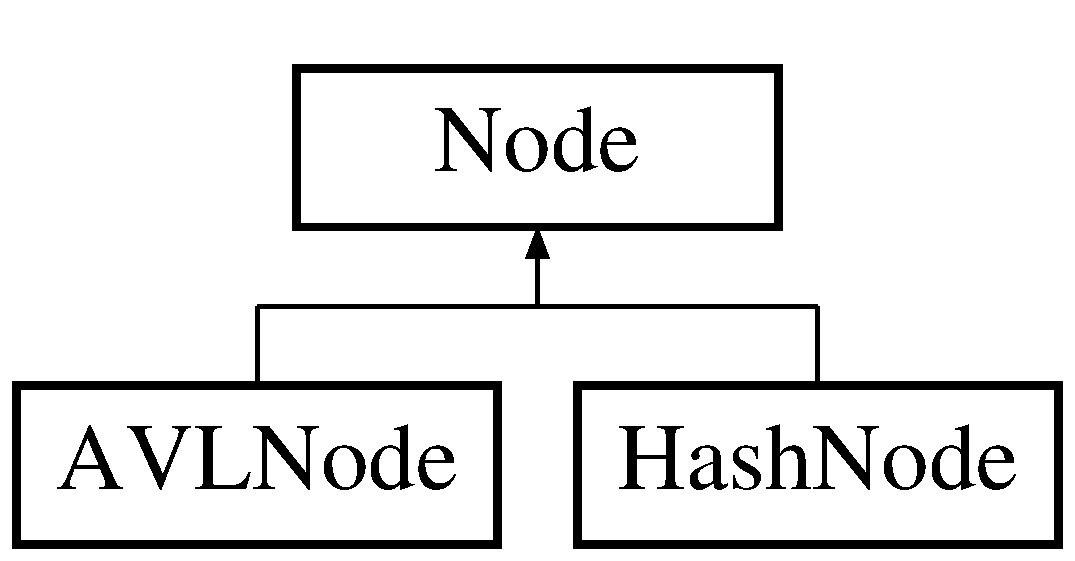
\includegraphics[height=2.000000cm]{class_node}
\end{center}
\end{figure}
\subsection*{Public Member Functions}
\begin{DoxyCompactItemize}
\item 
\hypertarget{class_node_a521cc0c4ebb153869947b76df9e0eada}{{\bfseries Node} (\hyperlink{class_page}{Page} $\ast$, string)}\label{class_node_a521cc0c4ebb153869947b76df9e0eada}

\item 
\hypertarget{class_node_ac5298373555f67634e27e5c739e7c94b}{string {\bfseries get\+Name} ()}\label{class_node_ac5298373555f67634e27e5c739e7c94b}

\item 
\hypertarget{class_node_a1fa90b3fa1a6ad3bbe616c4a6c0ba831}{set$<$ \hyperlink{class_page}{Page} $\ast$ $>$ {\bfseries get\+Set\+Of\+Pages} ()}\label{class_node_a1fa90b3fa1a6ad3bbe616c4a6c0ba831}

\item 
\hypertarget{class_node_ac6ab8994f203f84c076602540f003f7c}{void {\bfseries set\+Word} (string)}\label{class_node_ac6ab8994f203f84c076602540f003f7c}

\item 
\hypertarget{class_node_a742fe1af9dc4e51b0153a430bf2761bf}{set$<$ \hyperlink{class_page}{Page} $\ast$ $>$ {\bfseries get\+Binder} ()}\label{class_node_a742fe1af9dc4e51b0153a430bf2761bf}

\item 
\hypertarget{class_node_a921c6be0a1bb9c49ecaecaf675cd7260}{string {\bfseries get\+Word} ()}\label{class_node_a921c6be0a1bb9c49ecaecaf675cd7260}

\item 
\hypertarget{class_node_a2e469c97259b2823f9d9611da3ae2184}{void {\bfseries add\+To\+Binder} (\hyperlink{class_page}{Page} $\ast$\&)}\label{class_node_a2e469c97259b2823f9d9611da3ae2184}

\end{DoxyCompactItemize}


The documentation for this class was generated from the following files\+:\begin{DoxyCompactItemize}
\item 
Node.\+h\item 
Node.\+cpp\end{DoxyCompactItemize}

\hypertarget{class_page}{}\section{Page Class Reference}
\label{class_page}\index{Page@{Page}}


{\ttfamily \#include $<$Page.\+h$>$}

\subsection*{Public Member Functions}
\begin{DoxyCompactItemize}
\item 
\hyperlink{class_page_a9a7cc22d5459498ce638c54ae966c79b}{Page} ()
\item 
void \hyperlink{class_page_acf477f6eb17bab9955041f62cf773e8d}{set\+Title} (string)
\item 
void \hyperlink{class_page_ac482ec0d499e8c4d61f65bec3c845e05}{set\+Id} (unsigned long)
\item 
void \hyperlink{class_page_aa035203c86eb29a7121987ef5bfa1faf}{set\+Contributing\+User} (string)
\item 
void \hyperlink{class_page_a12df427d5f2620b2e912590eb1c81d32}{set\+Date} (string)
\item 
void \hyperlink{class_page_ada78e7ad8b4111afa5dd503151946e70}{set\+Frequency} (int, int)
\item 
void \hyperlink{class_page_a3f82c5cc09e31dc064246984ce7b7c17}{set\+Full\+Text} (string)
\item 
string \hyperlink{class_page_ad9647bb36d7587217dae9039aaf9d0db}{get\+Full\+Text} ()
\item 
string \hyperlink{class_page_ad8984dc2ec1c9d62343e35724080ee46}{get\+Title} ()
\item 
unsigned long \hyperlink{class_page_a8ce274bdff4b0f02131b0142dfd38dde}{get\+Id} ()
\item 
string \hyperlink{class_page_aa21e1e663df6f64d0670f4f9ac97330c}{get\+Contributing\+User} ()
\item 
string \hyperlink{class_page_aa9f674aaecb16f3ef02d54d0e42abe49}{get\+Date} ()
\item 
vector$<$ string $>$ \hyperlink{class_page_a31af27b5aa8f44f6bfb95fdbf555477c}{get\+Keywords} ()
\item 
int \hyperlink{class_page_a34588144ffb1c839e179f43aa7d9977c}{get\+Frequency} (int)
\item 
string \hyperlink{class_page_a0b43e8cd80b96011df19d083e6436a0f}{get\+Keyword\+At\+Index} (int)
\item 
void \hyperlink{class_page_a5650ea40b701dd7e15c7aa90fc819358}{increment\+Freq} (int)
\item 
int \hyperlink{class_page_a16d01583e3275c3a3c30793408f9865f}{add\+Keyword} (string \&)
\item 
\hyperlink{class_page_a2341fff1cc032ab6528874175e7dd841}{$\sim$\+Page} ()
\end{DoxyCompactItemize}
\subsection*{Static Public Member Functions}
\begin{DoxyCompactItemize}
\item 
static int \hyperlink{class_page_a8f1ef6fe4e22e67941a00bb6f5ff4be4}{binary\+Search} (vector$<$ string $>$ \&, string, int, int)
\end{DoxyCompactItemize}
\subsection*{Public Attributes}
\begin{DoxyCompactItemize}
\item 
string \hyperlink{class_page_a8713192624b3bc969533e4ebd39516c3}{full\+Text}
\end{DoxyCompactItemize}


\subsection{Constructor \& Destructor Documentation}
\hypertarget{class_page_a9a7cc22d5459498ce638c54ae966c79b}{}\index{Page@{Page}!Page@{Page}}
\index{Page@{Page}!Page@{Page}}
\subsubsection[{Page}]{\setlength{\rightskip}{0pt plus 5cm}Page\+::\+Page (
\begin{DoxyParamCaption}
{}
\end{DoxyParamCaption}
)}\label{class_page_a9a7cc22d5459498ce638c54ae966c79b}
\hypertarget{class_page_a2341fff1cc032ab6528874175e7dd841}{}\index{Page@{Page}!````~Page@{$\sim$\+Page}}
\index{````~Page@{$\sim$\+Page}!Page@{Page}}
\subsubsection[{$\sim$\+Page}]{\setlength{\rightskip}{0pt plus 5cm}Page\+::$\sim$\+Page (
\begin{DoxyParamCaption}
{}
\end{DoxyParamCaption}
)}\label{class_page_a2341fff1cc032ab6528874175e7dd841}


\subsection{Member Function Documentation}
\hypertarget{class_page_a16d01583e3275c3a3c30793408f9865f}{}\index{Page@{Page}!add\+Keyword@{add\+Keyword}}
\index{add\+Keyword@{add\+Keyword}!Page@{Page}}
\subsubsection[{add\+Keyword}]{\setlength{\rightskip}{0pt plus 5cm}int Page\+::add\+Keyword (
\begin{DoxyParamCaption}
\item[{string \&}]{keyword}
\end{DoxyParamCaption}
)}\label{class_page_a16d01583e3275c3a3c30793408f9865f}
\hypertarget{class_page_a8f1ef6fe4e22e67941a00bb6f5ff4be4}{}\index{Page@{Page}!binary\+Search@{binary\+Search}}
\index{binary\+Search@{binary\+Search}!Page@{Page}}
\subsubsection[{binary\+Search}]{\setlength{\rightskip}{0pt plus 5cm}int Page\+::binary\+Search (
\begin{DoxyParamCaption}
\item[{vector$<$ string $>$ \&}]{vc, }
\item[{string}]{kw, }
\item[{int}]{low, }
\item[{int}]{high}
\end{DoxyParamCaption}
)\hspace{0.3cm}{\ttfamily [static]}}\label{class_page_a8f1ef6fe4e22e67941a00bb6f5ff4be4}
\hypertarget{class_page_aa21e1e663df6f64d0670f4f9ac97330c}{}\index{Page@{Page}!get\+Contributing\+User@{get\+Contributing\+User}}
\index{get\+Contributing\+User@{get\+Contributing\+User}!Page@{Page}}
\subsubsection[{get\+Contributing\+User}]{\setlength{\rightskip}{0pt plus 5cm}string Page\+::get\+Contributing\+User (
\begin{DoxyParamCaption}
{}
\end{DoxyParamCaption}
)}\label{class_page_aa21e1e663df6f64d0670f4f9ac97330c}
\hypertarget{class_page_aa9f674aaecb16f3ef02d54d0e42abe49}{}\index{Page@{Page}!get\+Date@{get\+Date}}
\index{get\+Date@{get\+Date}!Page@{Page}}
\subsubsection[{get\+Date}]{\setlength{\rightskip}{0pt plus 5cm}string Page\+::get\+Date (
\begin{DoxyParamCaption}
{}
\end{DoxyParamCaption}
)}\label{class_page_aa9f674aaecb16f3ef02d54d0e42abe49}
\hypertarget{class_page_a34588144ffb1c839e179f43aa7d9977c}{}\index{Page@{Page}!get\+Frequency@{get\+Frequency}}
\index{get\+Frequency@{get\+Frequency}!Page@{Page}}
\subsubsection[{get\+Frequency}]{\setlength{\rightskip}{0pt plus 5cm}int Page\+::get\+Frequency (
\begin{DoxyParamCaption}
\item[{int}]{index}
\end{DoxyParamCaption}
)}\label{class_page_a34588144ffb1c839e179f43aa7d9977c}
\hypertarget{class_page_ad9647bb36d7587217dae9039aaf9d0db}{}\index{Page@{Page}!get\+Full\+Text@{get\+Full\+Text}}
\index{get\+Full\+Text@{get\+Full\+Text}!Page@{Page}}
\subsubsection[{get\+Full\+Text}]{\setlength{\rightskip}{0pt plus 5cm}string Page\+::get\+Full\+Text (
\begin{DoxyParamCaption}
{}
\end{DoxyParamCaption}
)}\label{class_page_ad9647bb36d7587217dae9039aaf9d0db}
\hypertarget{class_page_a8ce274bdff4b0f02131b0142dfd38dde}{}\index{Page@{Page}!get\+Id@{get\+Id}}
\index{get\+Id@{get\+Id}!Page@{Page}}
\subsubsection[{get\+Id}]{\setlength{\rightskip}{0pt plus 5cm}unsigned long Page\+::get\+Id (
\begin{DoxyParamCaption}
{}
\end{DoxyParamCaption}
)}\label{class_page_a8ce274bdff4b0f02131b0142dfd38dde}
\hypertarget{class_page_a0b43e8cd80b96011df19d083e6436a0f}{}\index{Page@{Page}!get\+Keyword\+At\+Index@{get\+Keyword\+At\+Index}}
\index{get\+Keyword\+At\+Index@{get\+Keyword\+At\+Index}!Page@{Page}}
\subsubsection[{get\+Keyword\+At\+Index}]{\setlength{\rightskip}{0pt plus 5cm}string Page\+::get\+Keyword\+At\+Index (
\begin{DoxyParamCaption}
\item[{int}]{index}
\end{DoxyParamCaption}
)}\label{class_page_a0b43e8cd80b96011df19d083e6436a0f}
\hypertarget{class_page_a31af27b5aa8f44f6bfb95fdbf555477c}{}\index{Page@{Page}!get\+Keywords@{get\+Keywords}}
\index{get\+Keywords@{get\+Keywords}!Page@{Page}}
\subsubsection[{get\+Keywords}]{\setlength{\rightskip}{0pt plus 5cm}vector$<$ string $>$ Page\+::get\+Keywords (
\begin{DoxyParamCaption}
{}
\end{DoxyParamCaption}
)}\label{class_page_a31af27b5aa8f44f6bfb95fdbf555477c}
\hypertarget{class_page_ad8984dc2ec1c9d62343e35724080ee46}{}\index{Page@{Page}!get\+Title@{get\+Title}}
\index{get\+Title@{get\+Title}!Page@{Page}}
\subsubsection[{get\+Title}]{\setlength{\rightskip}{0pt plus 5cm}string Page\+::get\+Title (
\begin{DoxyParamCaption}
{}
\end{DoxyParamCaption}
)}\label{class_page_ad8984dc2ec1c9d62343e35724080ee46}
\hypertarget{class_page_a5650ea40b701dd7e15c7aa90fc819358}{}\index{Page@{Page}!increment\+Freq@{increment\+Freq}}
\index{increment\+Freq@{increment\+Freq}!Page@{Page}}
\subsubsection[{increment\+Freq}]{\setlength{\rightskip}{0pt plus 5cm}void Page\+::increment\+Freq (
\begin{DoxyParamCaption}
\item[{int}]{index}
\end{DoxyParamCaption}
)}\label{class_page_a5650ea40b701dd7e15c7aa90fc819358}
\hypertarget{class_page_aa035203c86eb29a7121987ef5bfa1faf}{}\index{Page@{Page}!set\+Contributing\+User@{set\+Contributing\+User}}
\index{set\+Contributing\+User@{set\+Contributing\+User}!Page@{Page}}
\subsubsection[{set\+Contributing\+User}]{\setlength{\rightskip}{0pt plus 5cm}void Page\+::set\+Contributing\+User (
\begin{DoxyParamCaption}
\item[{string}]{username}
\end{DoxyParamCaption}
)}\label{class_page_aa035203c86eb29a7121987ef5bfa1faf}
\hypertarget{class_page_a12df427d5f2620b2e912590eb1c81d32}{}\index{Page@{Page}!set\+Date@{set\+Date}}
\index{set\+Date@{set\+Date}!Page@{Page}}
\subsubsection[{set\+Date}]{\setlength{\rightskip}{0pt plus 5cm}void Page\+::set\+Date (
\begin{DoxyParamCaption}
\item[{string}]{d}
\end{DoxyParamCaption}
)}\label{class_page_a12df427d5f2620b2e912590eb1c81d32}
\hypertarget{class_page_ada78e7ad8b4111afa5dd503151946e70}{}\index{Page@{Page}!set\+Frequency@{set\+Frequency}}
\index{set\+Frequency@{set\+Frequency}!Page@{Page}}
\subsubsection[{set\+Frequency}]{\setlength{\rightskip}{0pt plus 5cm}void Page\+::set\+Frequency (
\begin{DoxyParamCaption}
\item[{int}]{index, }
\item[{int}]{freq}
\end{DoxyParamCaption}
)}\label{class_page_ada78e7ad8b4111afa5dd503151946e70}
\hypertarget{class_page_a3f82c5cc09e31dc064246984ce7b7c17}{}\index{Page@{Page}!set\+Full\+Text@{set\+Full\+Text}}
\index{set\+Full\+Text@{set\+Full\+Text}!Page@{Page}}
\subsubsection[{set\+Full\+Text}]{\setlength{\rightskip}{0pt plus 5cm}void Page\+::set\+Full\+Text (
\begin{DoxyParamCaption}
\item[{string}]{text}
\end{DoxyParamCaption}
)}\label{class_page_a3f82c5cc09e31dc064246984ce7b7c17}
\hypertarget{class_page_ac482ec0d499e8c4d61f65bec3c845e05}{}\index{Page@{Page}!set\+Id@{set\+Id}}
\index{set\+Id@{set\+Id}!Page@{Page}}
\subsubsection[{set\+Id}]{\setlength{\rightskip}{0pt plus 5cm}void Page\+::set\+Id (
\begin{DoxyParamCaption}
\item[{unsigned long}]{num}
\end{DoxyParamCaption}
)}\label{class_page_ac482ec0d499e8c4d61f65bec3c845e05}
\hypertarget{class_page_acf477f6eb17bab9955041f62cf773e8d}{}\index{Page@{Page}!set\+Title@{set\+Title}}
\index{set\+Title@{set\+Title}!Page@{Page}}
\subsubsection[{set\+Title}]{\setlength{\rightskip}{0pt plus 5cm}void Page\+::set\+Title (
\begin{DoxyParamCaption}
\item[{string}]{t}
\end{DoxyParamCaption}
)}\label{class_page_acf477f6eb17bab9955041f62cf773e8d}


\subsection{Member Data Documentation}
\hypertarget{class_page_a8713192624b3bc969533e4ebd39516c3}{}\index{Page@{Page}!full\+Text@{full\+Text}}
\index{full\+Text@{full\+Text}!Page@{Page}}
\subsubsection[{full\+Text}]{\setlength{\rightskip}{0pt plus 5cm}string Page\+::full\+Text}\label{class_page_a8713192624b3bc969533e4ebd39516c3}


The documentation for this class was generated from the following files\+:\begin{DoxyCompactItemize}
\item 
\hyperlink{_page_8h}{Page.\+h}\item 
\hyperlink{_page_8cpp}{Page.\+cpp}\end{DoxyCompactItemize}

\hypertarget{class_query}{}\section{Query Class Reference}
\label{class_query}\index{Query@{Query}}


{\ttfamily \#include $<$Query.\+h$>$}

\subsection*{Public Member Functions}
\begin{DoxyCompactItemize}
\item 
\hyperlink{class_query_a4c1633236bdb9fa8d3fd3572a469889d}{Query} ()
\item 
std\+::vector$<$ std\+::string $>$ \hyperlink{class_query_a509091fc6e1bba8544991403a6d7b4b7}{getand\+Args} ()
\item 
std\+::vector$<$ std\+::string $>$ \hyperlink{class_query_ab90fc81524045a085b472dad8e6032bd}{getor\+Args} ()
\item 
std\+::vector$<$ std\+::string $>$ \hyperlink{class_query_a83014fdd314c75564ef1746fccd77407}{getnot\+Args} ()
\item 
std\+::vector$<$ std\+::string $>$ \hyperlink{class_query_afed0bd695e2b355d42ae78a79c2b2592}{getnorm\+Args} ()
\item 
std\+::string \hyperlink{class_query_aa2e86853eac7f292d4894cf8ef4260b0}{getand\+Args} (int)
\item 
std\+::string \hyperlink{class_query_ae3966de9b3bdba292a67b0e418a9d146}{getor\+Args} (int)
\item 
std\+::string \hyperlink{class_query_a7ef802901ce6e3b7b68e46b2f6659b18}{getnot\+Args} (int)
\item 
std\+::string \hyperlink{class_query_aa7d5b960f0d1cd7c83b7d191ac371d0a}{getnorm\+Args} (int)
\item 
void \hyperlink{class_query_a0497175553ef811642c5b2b3c0bd1ca2}{setand\+Args} (int, std\+::string)
\item 
void \hyperlink{class_query_afb2f5f87786fc282fefface523a81138}{setor\+Args} (int, std\+::string)
\item 
void \hyperlink{class_query_aef14c309f6f5880066f649a8f47fe3bc}{setnot\+Args} (int, std\+::string)
\item 
void \hyperlink{class_query_a24a65f32cdc1c1ee4246cbf480763557}{setnorm\+Args} (int, std\+::string)
\item 
void \hyperlink{class_query_a308104a6371bdf950435593413d527a6}{addand\+Args} (std\+::string)
\item 
void \hyperlink{class_query_aa19cc7a02d5e11c44118760bad4d0f50}{addor\+Args} (std\+::string)
\item 
void \hyperlink{class_query_a1923e0fdb1a976e23dc79731722d4fa3}{addnot\+Args} (std\+::string)
\item 
void \hyperlink{class_query_a038cf2204b03b09bd8423ee919c6866b}{addnorm\+Args} (std\+::string)
\item 
void \hyperlink{class_query_aa8b2a46725fdad4e06aad405b6c18227}{clear\+Query} ()
\item 
\hyperlink{class_query_aad0c964335e9809cc7e22af34e9e8410}{$\sim$\+Query} ()
\end{DoxyCompactItemize}


\subsection{Detailed Description}
\hyperlink{class_query}{Query} header file holds each keyword needing to be searched in query Sam Hunter and Morgan Monzingo 

\subsection{Constructor \& Destructor Documentation}
\hypertarget{class_query_a4c1633236bdb9fa8d3fd3572a469889d}{}\index{Query@{Query}!Query@{Query}}
\index{Query@{Query}!Query@{Query}}
\subsubsection[{Query}]{\setlength{\rightskip}{0pt plus 5cm}Query\+::\+Query (
\begin{DoxyParamCaption}
{}
\end{DoxyParamCaption}
)}\label{class_query_a4c1633236bdb9fa8d3fd3572a469889d}
\hypertarget{class_query_aad0c964335e9809cc7e22af34e9e8410}{}\index{Query@{Query}!````~Query@{$\sim$\+Query}}
\index{````~Query@{$\sim$\+Query}!Query@{Query}}
\subsubsection[{$\sim$\+Query}]{\setlength{\rightskip}{0pt plus 5cm}Query\+::$\sim$\+Query (
\begin{DoxyParamCaption}
{}
\end{DoxyParamCaption}
)}\label{class_query_aad0c964335e9809cc7e22af34e9e8410}


\subsection{Member Function Documentation}
\hypertarget{class_query_a308104a6371bdf950435593413d527a6}{}\index{Query@{Query}!addand\+Args@{addand\+Args}}
\index{addand\+Args@{addand\+Args}!Query@{Query}}
\subsubsection[{addand\+Args}]{\setlength{\rightskip}{0pt plus 5cm}void Query\+::addand\+Args (
\begin{DoxyParamCaption}
\item[{std\+::string}]{and\+Arg}
\end{DoxyParamCaption}
)}\label{class_query_a308104a6371bdf950435593413d527a6}
\hypertarget{class_query_a038cf2204b03b09bd8423ee919c6866b}{}\index{Query@{Query}!addnorm\+Args@{addnorm\+Args}}
\index{addnorm\+Args@{addnorm\+Args}!Query@{Query}}
\subsubsection[{addnorm\+Args}]{\setlength{\rightskip}{0pt plus 5cm}void Query\+::addnorm\+Args (
\begin{DoxyParamCaption}
\item[{std\+::string}]{norm\+Arg}
\end{DoxyParamCaption}
)}\label{class_query_a038cf2204b03b09bd8423ee919c6866b}
\hypertarget{class_query_a1923e0fdb1a976e23dc79731722d4fa3}{}\index{Query@{Query}!addnot\+Args@{addnot\+Args}}
\index{addnot\+Args@{addnot\+Args}!Query@{Query}}
\subsubsection[{addnot\+Args}]{\setlength{\rightskip}{0pt plus 5cm}void Query\+::addnot\+Args (
\begin{DoxyParamCaption}
\item[{std\+::string}]{}
\end{DoxyParamCaption}
)}\label{class_query_a1923e0fdb1a976e23dc79731722d4fa3}
\hypertarget{class_query_aa19cc7a02d5e11c44118760bad4d0f50}{}\index{Query@{Query}!addor\+Args@{addor\+Args}}
\index{addor\+Args@{addor\+Args}!Query@{Query}}
\subsubsection[{addor\+Args}]{\setlength{\rightskip}{0pt plus 5cm}void Query\+::addor\+Args (
\begin{DoxyParamCaption}
\item[{std\+::string}]{or\+Arg}
\end{DoxyParamCaption}
)}\label{class_query_aa19cc7a02d5e11c44118760bad4d0f50}
\hypertarget{class_query_aa8b2a46725fdad4e06aad405b6c18227}{}\index{Query@{Query}!clear\+Query@{clear\+Query}}
\index{clear\+Query@{clear\+Query}!Query@{Query}}
\subsubsection[{clear\+Query}]{\setlength{\rightskip}{0pt plus 5cm}void Query\+::clear\+Query (
\begin{DoxyParamCaption}
{}
\end{DoxyParamCaption}
)}\label{class_query_aa8b2a46725fdad4e06aad405b6c18227}
\hypertarget{class_query_a509091fc6e1bba8544991403a6d7b4b7}{}\index{Query@{Query}!getand\+Args@{getand\+Args}}
\index{getand\+Args@{getand\+Args}!Query@{Query}}
\subsubsection[{getand\+Args}]{\setlength{\rightskip}{0pt plus 5cm}std\+::vector$<$ std\+::string $>$ Query\+::getand\+Args (
\begin{DoxyParamCaption}
{}
\end{DoxyParamCaption}
)}\label{class_query_a509091fc6e1bba8544991403a6d7b4b7}
\hypertarget{class_query_aa2e86853eac7f292d4894cf8ef4260b0}{}\index{Query@{Query}!getand\+Args@{getand\+Args}}
\index{getand\+Args@{getand\+Args}!Query@{Query}}
\subsubsection[{getand\+Args}]{\setlength{\rightskip}{0pt plus 5cm}std\+::string Query\+::getand\+Args (
\begin{DoxyParamCaption}
\item[{int}]{index}
\end{DoxyParamCaption}
)}\label{class_query_aa2e86853eac7f292d4894cf8ef4260b0}
\hypertarget{class_query_afed0bd695e2b355d42ae78a79c2b2592}{}\index{Query@{Query}!getnorm\+Args@{getnorm\+Args}}
\index{getnorm\+Args@{getnorm\+Args}!Query@{Query}}
\subsubsection[{getnorm\+Args}]{\setlength{\rightskip}{0pt plus 5cm}std\+::vector$<$ std\+::string $>$ Query\+::getnorm\+Args (
\begin{DoxyParamCaption}
{}
\end{DoxyParamCaption}
)}\label{class_query_afed0bd695e2b355d42ae78a79c2b2592}
\hypertarget{class_query_aa7d5b960f0d1cd7c83b7d191ac371d0a}{}\index{Query@{Query}!getnorm\+Args@{getnorm\+Args}}
\index{getnorm\+Args@{getnorm\+Args}!Query@{Query}}
\subsubsection[{getnorm\+Args}]{\setlength{\rightskip}{0pt plus 5cm}std\+::string Query\+::getnorm\+Args (
\begin{DoxyParamCaption}
\item[{int}]{index}
\end{DoxyParamCaption}
)}\label{class_query_aa7d5b960f0d1cd7c83b7d191ac371d0a}
\hypertarget{class_query_a83014fdd314c75564ef1746fccd77407}{}\index{Query@{Query}!getnot\+Args@{getnot\+Args}}
\index{getnot\+Args@{getnot\+Args}!Query@{Query}}
\subsubsection[{getnot\+Args}]{\setlength{\rightskip}{0pt plus 5cm}std\+::vector$<$ std\+::string $>$ Query\+::getnot\+Args (
\begin{DoxyParamCaption}
{}
\end{DoxyParamCaption}
)}\label{class_query_a83014fdd314c75564ef1746fccd77407}
\hypertarget{class_query_a7ef802901ce6e3b7b68e46b2f6659b18}{}\index{Query@{Query}!getnot\+Args@{getnot\+Args}}
\index{getnot\+Args@{getnot\+Args}!Query@{Query}}
\subsubsection[{getnot\+Args}]{\setlength{\rightskip}{0pt plus 5cm}std\+::string Query\+::getnot\+Args (
\begin{DoxyParamCaption}
\item[{int}]{index}
\end{DoxyParamCaption}
)}\label{class_query_a7ef802901ce6e3b7b68e46b2f6659b18}
\hypertarget{class_query_ab90fc81524045a085b472dad8e6032bd}{}\index{Query@{Query}!getor\+Args@{getor\+Args}}
\index{getor\+Args@{getor\+Args}!Query@{Query}}
\subsubsection[{getor\+Args}]{\setlength{\rightskip}{0pt plus 5cm}std\+::vector$<$ std\+::string $>$ Query\+::getor\+Args (
\begin{DoxyParamCaption}
{}
\end{DoxyParamCaption}
)}\label{class_query_ab90fc81524045a085b472dad8e6032bd}
\hypertarget{class_query_ae3966de9b3bdba292a67b0e418a9d146}{}\index{Query@{Query}!getor\+Args@{getor\+Args}}
\index{getor\+Args@{getor\+Args}!Query@{Query}}
\subsubsection[{getor\+Args}]{\setlength{\rightskip}{0pt plus 5cm}std\+::string Query\+::getor\+Args (
\begin{DoxyParamCaption}
\item[{int}]{index}
\end{DoxyParamCaption}
)}\label{class_query_ae3966de9b3bdba292a67b0e418a9d146}
\hypertarget{class_query_a0497175553ef811642c5b2b3c0bd1ca2}{}\index{Query@{Query}!setand\+Args@{setand\+Args}}
\index{setand\+Args@{setand\+Args}!Query@{Query}}
\subsubsection[{setand\+Args}]{\setlength{\rightskip}{0pt plus 5cm}void Query\+::setand\+Args (
\begin{DoxyParamCaption}
\item[{int}]{index, }
\item[{std\+::string}]{new\+Word}
\end{DoxyParamCaption}
)}\label{class_query_a0497175553ef811642c5b2b3c0bd1ca2}
\hypertarget{class_query_a24a65f32cdc1c1ee4246cbf480763557}{}\index{Query@{Query}!setnorm\+Args@{setnorm\+Args}}
\index{setnorm\+Args@{setnorm\+Args}!Query@{Query}}
\subsubsection[{setnorm\+Args}]{\setlength{\rightskip}{0pt plus 5cm}void Query\+::setnorm\+Args (
\begin{DoxyParamCaption}
\item[{int}]{index, }
\item[{std\+::string}]{new\+Word}
\end{DoxyParamCaption}
)}\label{class_query_a24a65f32cdc1c1ee4246cbf480763557}
\hypertarget{class_query_aef14c309f6f5880066f649a8f47fe3bc}{}\index{Query@{Query}!setnot\+Args@{setnot\+Args}}
\index{setnot\+Args@{setnot\+Args}!Query@{Query}}
\subsubsection[{setnot\+Args}]{\setlength{\rightskip}{0pt plus 5cm}void Query\+::setnot\+Args (
\begin{DoxyParamCaption}
\item[{int}]{index, }
\item[{std\+::string}]{new\+Word}
\end{DoxyParamCaption}
)}\label{class_query_aef14c309f6f5880066f649a8f47fe3bc}
\hypertarget{class_query_afb2f5f87786fc282fefface523a81138}{}\index{Query@{Query}!setor\+Args@{setor\+Args}}
\index{setor\+Args@{setor\+Args}!Query@{Query}}
\subsubsection[{setor\+Args}]{\setlength{\rightskip}{0pt plus 5cm}void Query\+::setor\+Args (
\begin{DoxyParamCaption}
\item[{int}]{index, }
\item[{std\+::string}]{new\+Word}
\end{DoxyParamCaption}
)}\label{class_query_afb2f5f87786fc282fefface523a81138}


The documentation for this class was generated from the following files\+:\begin{DoxyCompactItemize}
\item 
\hyperlink{_query_8h}{Query.\+h}\item 
\hyperlink{_query_8cpp}{Query.\+cpp}\end{DoxyCompactItemize}

\hypertarget{class_query_processor}{\section{Query\+Processor Class Reference}
\label{class_query_processor}\index{Query\+Processor@{Query\+Processor}}
}
\subsection*{Public Member Functions}
\begin{DoxyCompactItemize}
\item 
\hypertarget{class_query_processor_a87834efeca2f9af6e32fb5a545d33067}{void {\bfseries parse\+Query} (std\+::string)}\label{class_query_processor_a87834efeca2f9af6e32fb5a545d33067}

\item 
\hypertarget{class_query_processor_a5b1b684b03f82b2ef8137ce630be7c33}{void {\bfseries not\+Arg\+Finder} (int)}\label{class_query_processor_a5b1b684b03f82b2ef8137ce630be7c33}

\item 
\hypertarget{class_query_processor_af6b62a64663cd688f4a55d66570a28a2}{void {\bfseries other\+Arg\+Finder} (int)}\label{class_query_processor_af6b62a64663cd688f4a55d66570a28a2}

\item 
\hypertarget{class_query_processor_a00cadfdc04ae5a048c58cbd9e7eebb1a}{void {\bfseries stem\+Query} ()}\label{class_query_processor_a00cadfdc04ae5a048c58cbd9e7eebb1a}

\item 
\hypertarget{class_query_processor_abc27ce568c2aa6cd84cfc10bca4b803b}{void {\bfseries print} ()}\label{class_query_processor_abc27ce568c2aa6cd84cfc10bca4b803b}

\end{DoxyCompactItemize}


The documentation for this class was generated from the following files\+:\begin{DoxyCompactItemize}
\item 
Query\+Processor.\+h\item 
Query\+Processor.\+cpp\end{DoxyCompactItemize}

\hypertarget{class_result}{}\section{Result Class Reference}
\label{class_result}\index{Result@{Result}}


{\ttfamily \#include $<$Result.\+h$>$}

\subsection*{Public Member Functions}
\begin{DoxyCompactItemize}
\item 
\hyperlink{class_result_a90f44667e23d25ccdeac37f00a74657b}{Result} ()
\item 
\hyperlink{class_result_aa9af2598d5c67a6f2b9b7f62a8bdef5f}{Result} (\hyperlink{class_page}{Page} $\ast$info, double inv\+Freq)
\item 
\hyperlink{class_result_ae11b1bc4250c6635e479feacc6e57143}{Result} (\hyperlink{class_page}{Page} $\ast$info, double inv\+Freq, string full)
\item 
void \hyperlink{class_result_abddeaa3ab93737073bc1b4463db2a0cc}{add\+Full\+Text} (string text)
\item 
int \hyperlink{class_result_a6e4b4fd6e92552928b89e9cd69ac0293}{get\+Id} ()
\item 
string \hyperlink{class_result_ad9754f0a6a069b60f259839010b7c085}{get\+Title} ()
\item 
\hyperlink{class_page}{Page} $\ast$ \hyperlink{class_result_a8cc69e34663f949bd9e99896e8ebba32}{get\+Page} ()
\item 
double \hyperlink{class_result_ac8510240d19e05e57cbfd3a3c5333677}{get\+Inverse\+Frequency} ()
\item 
string \hyperlink{class_result_ab4bfba7f8a8201f0ff6ee60eeed3cc04}{get\+Full\+Text} ()
\item 
string \hyperlink{class_result_a2f4828c3d73fe71e00ecafe7fa4a88fa}{get\+Date} ()
\end{DoxyCompactItemize}


\subsection{Constructor \& Destructor Documentation}
\hypertarget{class_result_a90f44667e23d25ccdeac37f00a74657b}{}\index{Result@{Result}!Result@{Result}}
\index{Result@{Result}!Result@{Result}}
\subsubsection[{Result}]{\setlength{\rightskip}{0pt plus 5cm}Result\+::\+Result (
\begin{DoxyParamCaption}
{}
\end{DoxyParamCaption}
)\hspace{0.3cm}{\ttfamily [inline]}}\label{class_result_a90f44667e23d25ccdeac37f00a74657b}
\hypertarget{class_result_aa9af2598d5c67a6f2b9b7f62a8bdef5f}{}\index{Result@{Result}!Result@{Result}}
\index{Result@{Result}!Result@{Result}}
\subsubsection[{Result}]{\setlength{\rightskip}{0pt plus 5cm}Result\+::\+Result (
\begin{DoxyParamCaption}
\item[{{\bf Page} $\ast$}]{info, }
\item[{double}]{inv\+Freq}
\end{DoxyParamCaption}
)\hspace{0.3cm}{\ttfamily [inline]}}\label{class_result_aa9af2598d5c67a6f2b9b7f62a8bdef5f}
\hypertarget{class_result_ae11b1bc4250c6635e479feacc6e57143}{}\index{Result@{Result}!Result@{Result}}
\index{Result@{Result}!Result@{Result}}
\subsubsection[{Result}]{\setlength{\rightskip}{0pt plus 5cm}Result\+::\+Result (
\begin{DoxyParamCaption}
\item[{{\bf Page} $\ast$}]{info, }
\item[{double}]{inv\+Freq, }
\item[{string}]{full}
\end{DoxyParamCaption}
)\hspace{0.3cm}{\ttfamily [inline]}}\label{class_result_ae11b1bc4250c6635e479feacc6e57143}


\subsection{Member Function Documentation}
\hypertarget{class_result_abddeaa3ab93737073bc1b4463db2a0cc}{}\index{Result@{Result}!add\+Full\+Text@{add\+Full\+Text}}
\index{add\+Full\+Text@{add\+Full\+Text}!Result@{Result}}
\subsubsection[{add\+Full\+Text}]{\setlength{\rightskip}{0pt plus 5cm}void Result\+::add\+Full\+Text (
\begin{DoxyParamCaption}
\item[{string}]{text}
\end{DoxyParamCaption}
)\hspace{0.3cm}{\ttfamily [inline]}}\label{class_result_abddeaa3ab93737073bc1b4463db2a0cc}
\hypertarget{class_result_a2f4828c3d73fe71e00ecafe7fa4a88fa}{}\index{Result@{Result}!get\+Date@{get\+Date}}
\index{get\+Date@{get\+Date}!Result@{Result}}
\subsubsection[{get\+Date}]{\setlength{\rightskip}{0pt plus 5cm}string Result\+::get\+Date (
\begin{DoxyParamCaption}
{}
\end{DoxyParamCaption}
)\hspace{0.3cm}{\ttfamily [inline]}}\label{class_result_a2f4828c3d73fe71e00ecafe7fa4a88fa}
\hypertarget{class_result_ab4bfba7f8a8201f0ff6ee60eeed3cc04}{}\index{Result@{Result}!get\+Full\+Text@{get\+Full\+Text}}
\index{get\+Full\+Text@{get\+Full\+Text}!Result@{Result}}
\subsubsection[{get\+Full\+Text}]{\setlength{\rightskip}{0pt plus 5cm}string Result\+::get\+Full\+Text (
\begin{DoxyParamCaption}
{}
\end{DoxyParamCaption}
)\hspace{0.3cm}{\ttfamily [inline]}}\label{class_result_ab4bfba7f8a8201f0ff6ee60eeed3cc04}
\hypertarget{class_result_a6e4b4fd6e92552928b89e9cd69ac0293}{}\index{Result@{Result}!get\+Id@{get\+Id}}
\index{get\+Id@{get\+Id}!Result@{Result}}
\subsubsection[{get\+Id}]{\setlength{\rightskip}{0pt plus 5cm}int Result\+::get\+Id (
\begin{DoxyParamCaption}
{}
\end{DoxyParamCaption}
)\hspace{0.3cm}{\ttfamily [inline]}}\label{class_result_a6e4b4fd6e92552928b89e9cd69ac0293}
\hypertarget{class_result_ac8510240d19e05e57cbfd3a3c5333677}{}\index{Result@{Result}!get\+Inverse\+Frequency@{get\+Inverse\+Frequency}}
\index{get\+Inverse\+Frequency@{get\+Inverse\+Frequency}!Result@{Result}}
\subsubsection[{get\+Inverse\+Frequency}]{\setlength{\rightskip}{0pt plus 5cm}double Result\+::get\+Inverse\+Frequency (
\begin{DoxyParamCaption}
{}
\end{DoxyParamCaption}
)\hspace{0.3cm}{\ttfamily [inline]}}\label{class_result_ac8510240d19e05e57cbfd3a3c5333677}
\hypertarget{class_result_a8cc69e34663f949bd9e99896e8ebba32}{}\index{Result@{Result}!get\+Page@{get\+Page}}
\index{get\+Page@{get\+Page}!Result@{Result}}
\subsubsection[{get\+Page}]{\setlength{\rightskip}{0pt plus 5cm}{\bf Page}$\ast$ Result\+::get\+Page (
\begin{DoxyParamCaption}
{}
\end{DoxyParamCaption}
)\hspace{0.3cm}{\ttfamily [inline]}}\label{class_result_a8cc69e34663f949bd9e99896e8ebba32}
\hypertarget{class_result_ad9754f0a6a069b60f259839010b7c085}{}\index{Result@{Result}!get\+Title@{get\+Title}}
\index{get\+Title@{get\+Title}!Result@{Result}}
\subsubsection[{get\+Title}]{\setlength{\rightskip}{0pt plus 5cm}string Result\+::get\+Title (
\begin{DoxyParamCaption}
{}
\end{DoxyParamCaption}
)\hspace{0.3cm}{\ttfamily [inline]}}\label{class_result_ad9754f0a6a069b60f259839010b7c085}


The documentation for this class was generated from the following file\+:\begin{DoxyCompactItemize}
\item 
\hyperlink{_result_8h}{Result.\+h}\end{DoxyCompactItemize}

\hypertarget{class_stem_helper}{}\section{Stem\+Helper Class Reference}
\label{class_stem_helper}\index{Stem\+Helper@{Stem\+Helper}}


{\ttfamily \#include $<$stem\+Helper.\+h$>$}

\subsection*{Static Public Member Functions}
\begin{DoxyCompactItemize}
\item 
static std\+::string \hyperlink{class_stem_helper_af2878d595387afb436bb38ae0a1c9f4d}{stemword} (char $\ast$buffer)
\end{DoxyCompactItemize}


\subsection{Member Function Documentation}
\hypertarget{class_stem_helper_af2878d595387afb436bb38ae0a1c9f4d}{}\index{Stem\+Helper@{Stem\+Helper}!stemword@{stemword}}
\index{stemword@{stemword}!Stem\+Helper@{Stem\+Helper}}
\subsubsection[{stemword}]{\setlength{\rightskip}{0pt plus 5cm}static std\+::string Stem\+Helper\+::stemword (
\begin{DoxyParamCaption}
\item[{char $\ast$}]{buffer}
\end{DoxyParamCaption}
)\hspace{0.3cm}{\ttfamily [inline]}, {\ttfamily [static]}}\label{class_stem_helper_af2878d595387afb436bb38ae0a1c9f4d}


The documentation for this class was generated from the following file\+:\begin{DoxyCompactItemize}
\item 
\hyperlink{stem_helper_8h}{stem\+Helper.\+h}\end{DoxyCompactItemize}

\hypertarget{structstemmer}{}\section{stemmer Struct Reference}
\label{structstemmer}\index{stemmer@{stemmer}}


{\ttfamily \#include $<$Porter\+Stemmer.\+h$>$}

\subsection*{Public Attributes}
\begin{DoxyCompactItemize}
\item 
char $\ast$ \hyperlink{structstemmer_a0ae99db94786418a0c4d85a2a15382a5}{b}
\item 
int \hyperlink{structstemmer_a587d5f8fd5c491688bc91e7d3b5e262e}{k}
\item 
int \hyperlink{structstemmer_a024d42a47e06bd5207e2494cbfefbf2f}{j}
\end{DoxyCompactItemize}


\subsection{Member Data Documentation}
\hypertarget{structstemmer_a0ae99db94786418a0c4d85a2a15382a5}{}\index{stemmer@{stemmer}!b@{b}}
\index{b@{b}!stemmer@{stemmer}}
\subsubsection[{b}]{\setlength{\rightskip}{0pt plus 5cm}char$\ast$ stemmer\+::b}\label{structstemmer_a0ae99db94786418a0c4d85a2a15382a5}
\hypertarget{structstemmer_a024d42a47e06bd5207e2494cbfefbf2f}{}\index{stemmer@{stemmer}!j@{j}}
\index{j@{j}!stemmer@{stemmer}}
\subsubsection[{j}]{\setlength{\rightskip}{0pt plus 5cm}int stemmer\+::j}\label{structstemmer_a024d42a47e06bd5207e2494cbfefbf2f}
\hypertarget{structstemmer_a587d5f8fd5c491688bc91e7d3b5e262e}{}\index{stemmer@{stemmer}!k@{k}}
\index{k@{k}!stemmer@{stemmer}}
\subsubsection[{k}]{\setlength{\rightskip}{0pt plus 5cm}int stemmer\+::k}\label{structstemmer_a587d5f8fd5c491688bc91e7d3b5e262e}


The documentation for this struct was generated from the following file\+:\begin{DoxyCompactItemize}
\item 
\hyperlink{_porter_stemmer_8h}{Porter\+Stemmer.\+h}\end{DoxyCompactItemize}

\hypertarget{class_user_interface}{\section{User\+Interface Class Reference}
\label{class_user_interface}\index{User\+Interface@{User\+Interface}}
}
\subsection*{Public Member Functions}
\begin{DoxyCompactItemize}
\item 
\hypertarget{class_user_interface_a5f668ba7e20441556650a2ab57919eb8}{void {\bfseries driver} ()}\label{class_user_interface_a5f668ba7e20441556650a2ab57919eb8}

\item 
\hypertarget{class_user_interface_aef424faaaab1a26e7e95615953dfb6b5}{void {\bfseries maintenence\+Mode} ()}\label{class_user_interface_aef424faaaab1a26e7e95615953dfb6b5}

\item 
\hypertarget{class_user_interface_a31406e8b5be6361c5e45f4f9b873c995}{void {\bfseries interactive\+Mode} ()}\label{class_user_interface_a31406e8b5be6361c5e45f4f9b873c995}

\item 
\hypertarget{class_user_interface_a0e9d6f1de4247604921f008ad8fd488b}{void {\bfseries stress\+Test} ()}\label{class_user_interface_a0e9d6f1de4247604921f008ad8fd488b}

\item 
\hypertarget{class_user_interface_a2b38e64d7c7cd64d09e8719ff747b244}{bool {\bfseries fexists} (const string \&)}\label{class_user_interface_a2b38e64d7c7cd64d09e8719ff747b244}

\item 
\hypertarget{class_user_interface_ac6235e19919c71faf514f82ae89b922f}{void {\bfseries clear\+Index} ()}\label{class_user_interface_ac6235e19919c71faf514f82ae89b922f}

\item 
\hypertarget{class_user_interface_a5aae71a73a68b9876c5ce7b1cba54910}{void {\bfseries add\+Files\+To\+Index} ()}\label{class_user_interface_a5aae71a73a68b9876c5ce7b1cba54910}

\item 
\hypertarget{class_user_interface_a6afb3103066951f4f3c69931cea544de}{void {\bfseries create\+Structure} (string)}\label{class_user_interface_a6afb3103066951f4f3c69931cea544de}

\item 
\hypertarget{class_user_interface_a141bf602a34bc9e85176bf05f3889ad2}{void {\bfseries add\+To\+Existing\+Index} ()}\label{class_user_interface_a141bf602a34bc9e85176bf05f3889ad2}

\end{DoxyCompactItemize}


The documentation for this class was generated from the following files\+:\begin{DoxyCompactItemize}
\item 
User\+Interface.\+h\item 
User\+Interface.\+cpp\end{DoxyCompactItemize}

\chapter{File Documentation}
\hypertarget{_a_v_l_node_8cpp}{}\section{A\+V\+L\+Node.\+cpp File Reference}
\label{_a_v_l_node_8cpp}\index{A\+V\+L\+Node.\+cpp@{A\+V\+L\+Node.\+cpp}}
{\ttfamily \#include \char`\"{}A\+V\+L\+Node.\+h\char`\"{}}\\*

\hypertarget{_a_v_l_node_8h}{}\section{A\+V\+L\+Node.\+h File Reference}
\label{_a_v_l_node_8h}\index{A\+V\+L\+Node.\+h@{A\+V\+L\+Node.\+h}}
{\ttfamily \#include $<$iostream$>$}\\*
{\ttfamily \#include \char`\"{}Node.\+h\char`\"{}}\\*
{\ttfamily \#include \char`\"{}Page.\+h\char`\"{}}\\*
\subsection*{Classes}
\begin{DoxyCompactItemize}
\item 
class \hyperlink{class_a_v_l_node}{A\+V\+L\+Node}
\end{DoxyCompactItemize}

\hypertarget{_a_v_l_tree_8cpp}{}\section{A\+V\+L\+Tree.\+cpp File Reference}
\label{_a_v_l_tree_8cpp}\index{A\+V\+L\+Tree.\+cpp@{A\+V\+L\+Tree.\+cpp}}
{\ttfamily \#include \char`\"{}A\+V\+L\+Tree.\+h\char`\"{}}\\*

\hypertarget{_a_v_l_tree_8h}{}\section{A\+V\+L\+Tree.\+h File Reference}
\label{_a_v_l_tree_8h}\index{A\+V\+L\+Tree.\+h@{A\+V\+L\+Tree.\+h}}
{\ttfamily \#include $<$iostream$>$}\\*
{\ttfamily \#include \char`\"{}Index\+Handler.\+h\char`\"{}}\\*
{\ttfamily \#include \char`\"{}A\+V\+L\+Node.\+h\char`\"{}}\\*
{\ttfamily \#include $<$cmath$>$}\\*
\subsection*{Classes}
\begin{DoxyCompactItemize}
\item 
class \hyperlink{class_a_v_l_tree}{A\+V\+L\+Tree}
\end{DoxyCompactItemize}

\hypertarget{_document_parser_8cpp}{}\section{Document\+Parser.\+cpp File Reference}
\label{_document_parser_8cpp}\index{Document\+Parser.\+cpp@{Document\+Parser.\+cpp}}
{\ttfamily \#include \char`\"{}Document\+Parser.\+h\char`\"{}}\\*
{\ttfamily \#include \char`\"{}stem\+Helper.\+h\char`\"{}}\\*

\hypertarget{_document_parser_8h}{}\section{Document\+Parser.\+h File Reference}
\label{_document_parser_8h}\index{Document\+Parser.\+h@{Document\+Parser.\+h}}
{\ttfamily \#include $<$fstream$>$}\\*
{\ttfamily \#include $<$vector$>$}\\*
{\ttfamily \#include \char`\"{}Page.\+h\char`\"{}}\\*
{\ttfamily \#include \char`\"{}Index\+Handler.\+h\char`\"{}}\\*
{\ttfamily \#include \char`\"{}Hash\+Table.\+h\char`\"{}}\\*
{\ttfamily \#include $<$algorithm$>$}\\*
{\ttfamily \#include $<$string$>$}\\*
{\ttfamily \#include $<$sstream$>$}\\*
{\ttfamily \#include $<$map$>$}\\*
{\ttfamily \#include $<$iostream$>$}\\*
{\ttfamily \#include $<$cctype$>$}\\*
\subsection*{Classes}
\begin{DoxyCompactItemize}
\item 
class \hyperlink{class_document_parser}{Document\+Parser}
\end{DoxyCompactItemize}

\hypertarget{_hash_node_8cpp}{}\section{Hash\+Node.\+cpp File Reference}
\label{_hash_node_8cpp}\index{Hash\+Node.\+cpp@{Hash\+Node.\+cpp}}
{\ttfamily \#include \char`\"{}Hash\+Node.\+h\char`\"{}}\\*

\hypertarget{_hash_node_8h}{}\section{Hash\+Node.\+h File Reference}
\label{_hash_node_8h}\index{Hash\+Node.\+h@{Hash\+Node.\+h}}
{\ttfamily \#include \char`\"{}Node.\+h\char`\"{}}\\*
\subsection*{Classes}
\begin{DoxyCompactItemize}
\item 
class \hyperlink{class_hash_node}{Hash\+Node}
\end{DoxyCompactItemize}

\hypertarget{_hash_table_8cpp}{}\section{Hash\+Table.\+cpp File Reference}
\label{_hash_table_8cpp}\index{Hash\+Table.\+cpp@{Hash\+Table.\+cpp}}
{\ttfamily \#include $<$iostream$>$}\\*
{\ttfamily \#include \char`\"{}Hash\+Table.\+h\char`\"{}}\\*
{\ttfamily \#include $<$functional$>$}\\*

\hypertarget{_hash_table_8h}{}\section{Hash\+Table.\+h File Reference}
\label{_hash_table_8h}\index{Hash\+Table.\+h@{Hash\+Table.\+h}}
{\ttfamily \#include $<$vector$>$}\\*
{\ttfamily \#include $<$set$>$}\\*
{\ttfamily \#include $<$iostream$>$}\\*
{\ttfamily \#include \char`\"{}Page.\+h\char`\"{}}\\*
{\ttfamily \#include \char`\"{}Node.\+h\char`\"{}}\\*
{\ttfamily \#include \char`\"{}Hash\+Node.\+h\char`\"{}}\\*
{\ttfamily \#include \char`\"{}Index\+Handler.\+h\char`\"{}}\\*
\subsection*{Classes}
\begin{DoxyCompactItemize}
\item 
class \hyperlink{class_hash_table}{Hash\+Table}
\end{DoxyCompactItemize}

\hypertarget{_index_handler_8cpp}{}\section{Index\+Handler.\+cpp File Reference}
\label{_index_handler_8cpp}\index{Index\+Handler.\+cpp@{Index\+Handler.\+cpp}}
{\ttfamily \#include \char`\"{}Index\+Handler.\+h\char`\"{}}\\*

\hypertarget{_index_handler_8h}{}\section{Index\+Handler.\+h File Reference}
\label{_index_handler_8h}\index{Index\+Handler.\+h@{Index\+Handler.\+h}}
{\ttfamily \#include $<$iostream$>$}\\*
{\ttfamily \#include \char`\"{}Page.\+h\char`\"{}}\\*
{\ttfamily \#include \char`\"{}Query.\+h\char`\"{}}\\*
{\ttfamily \#include $<$set$>$}\\*
{\ttfamily \#include $<$chrono$>$}\\*
\subsection*{Classes}
\begin{DoxyCompactItemize}
\item 
class \hyperlink{class_index_handler}{Index\+Handler}
\end{DoxyCompactItemize}

\hypertarget{main_8cpp}{}\section{main.\+cpp File Reference}
\label{main_8cpp}\index{main.\+cpp@{main.\+cpp}}
{\ttfamily \#include $<$fstream$>$}\\*
{\ttfamily \#include $<$iostream$>$}\\*
{\ttfamily \#include \char`\"{}Document\+Parser.\+h\char`\"{}}\\*
{\ttfamily \#include \char`\"{}Index\+Handler.\+h\char`\"{}}\\*
{\ttfamily \#include \char`\"{}A\+V\+L\+Tree.\+h\char`\"{}}\\*
{\ttfamily \#include \char`\"{}User\+Interface.\+h\char`\"{}}\\*
{\ttfamily \#include $<$iomanip$>$}\\*
{\ttfamily \#include \char`\"{}Query\+Processor.\+h\char`\"{}}\\*
\subsection*{Functions}
\begin{DoxyCompactItemize}
\item 
int \hyperlink{main_8cpp_ae66f6b31b5ad750f1fe042a706a4e3d4}{main} ()
\end{DoxyCompactItemize}


\subsection{Function Documentation}
\hypertarget{main_8cpp_ae66f6b31b5ad750f1fe042a706a4e3d4}{}\index{main.\+cpp@{main.\+cpp}!main@{main}}
\index{main@{main}!main.\+cpp@{main.\+cpp}}
\subsubsection[{main}]{\setlength{\rightskip}{0pt plus 5cm}int main (
\begin{DoxyParamCaption}
{}
\end{DoxyParamCaption}
)}\label{main_8cpp_ae66f6b31b5ad750f1fe042a706a4e3d4}

\hypertarget{_node_8cpp}{}\section{Node.\+cpp File Reference}
\label{_node_8cpp}\index{Node.\+cpp@{Node.\+cpp}}
{\ttfamily \#include \char`\"{}Node.\+h\char`\"{}}\\*

\hypertarget{_node_8h}{}\section{Node.\+h File Reference}
\label{_node_8h}\index{Node.\+h@{Node.\+h}}
{\ttfamily \#include $<$iostream$>$}\\*
{\ttfamily \#include $<$set$>$}\\*
{\ttfamily \#include \char`\"{}Page.\+h\char`\"{}}\\*
\subsection*{Classes}
\begin{DoxyCompactItemize}
\item 
class \hyperlink{class_node}{Node}
\end{DoxyCompactItemize}

\hypertarget{_page_8cpp}{}\section{Page.\+cpp File Reference}
\label{_page_8cpp}\index{Page.\+cpp@{Page.\+cpp}}
{\ttfamily \#include \char`\"{}Page.\+h\char`\"{}}\\*

\hypertarget{_page_8h}{}\section{Page.\+h File Reference}
\label{_page_8h}\index{Page.\+h@{Page.\+h}}
{\ttfamily \#include $<$iostream$>$}\\*
{\ttfamily \#include $<$vector$>$}\\*
{\ttfamily \#include $<$string$>$}\\*
\subsection*{Classes}
\begin{DoxyCompactItemize}
\item 
class \hyperlink{class_page}{Page}
\end{DoxyCompactItemize}

\hypertarget{_porter_stemmer_8h}{}\section{Porter\+Stemmer.\+h File Reference}
\label{_porter_stemmer_8h}\index{Porter\+Stemmer.\+h@{Porter\+Stemmer.\+h}}
{\ttfamily \#include $<$cstdlib$>$}\\*
{\ttfamily \#include $<$cstring$>$}\\*
\subsection*{Classes}
\begin{DoxyCompactItemize}
\item 
struct \hyperlink{structstemmer}{stemmer}
\end{DoxyCompactItemize}
\subsection*{Macros}
\begin{DoxyCompactItemize}
\item 
\#define \hyperlink{_porter_stemmer_8h_aa8cecfc5c5c054d2875c03e77b7be15d}{T\+R\+U\+E}~1
\item 
\#define \hyperlink{_porter_stemmer_8h_aa93f0eb578d23995850d61f7d61c55c1}{F\+A\+L\+S\+E}~0
\end{DoxyCompactItemize}


\subsection{Macro Definition Documentation}
\hypertarget{_porter_stemmer_8h_aa93f0eb578d23995850d61f7d61c55c1}{}\index{Porter\+Stemmer.\+h@{Porter\+Stemmer.\+h}!F\+A\+L\+S\+E@{F\+A\+L\+S\+E}}
\index{F\+A\+L\+S\+E@{F\+A\+L\+S\+E}!Porter\+Stemmer.\+h@{Porter\+Stemmer.\+h}}
\subsubsection[{F\+A\+L\+S\+E}]{\setlength{\rightskip}{0pt plus 5cm}\#define F\+A\+L\+S\+E~0}\label{_porter_stemmer_8h_aa93f0eb578d23995850d61f7d61c55c1}
\hypertarget{_porter_stemmer_8h_aa8cecfc5c5c054d2875c03e77b7be15d}{}\index{Porter\+Stemmer.\+h@{Porter\+Stemmer.\+h}!T\+R\+U\+E@{T\+R\+U\+E}}
\index{T\+R\+U\+E@{T\+R\+U\+E}!Porter\+Stemmer.\+h@{Porter\+Stemmer.\+h}}
\subsubsection[{T\+R\+U\+E}]{\setlength{\rightskip}{0pt plus 5cm}\#define T\+R\+U\+E~1}\label{_porter_stemmer_8h_aa8cecfc5c5c054d2875c03e77b7be15d}

\hypertarget{_query_8cpp}{}\section{Query.\+cpp File Reference}
\label{_query_8cpp}\index{Query.\+cpp@{Query.\+cpp}}
{\ttfamily \#include \char`\"{}Query.\+h\char`\"{}}\\*

\hypertarget{_query_8h}{}\section{Query.\+h File Reference}
\label{_query_8h}\index{Query.\+h@{Query.\+h}}
{\ttfamily \#include $<$vector$>$}\\*
{\ttfamily \#include $<$string$>$}\\*
{\ttfamily \#include $<$iostream$>$}\\*
\subsection*{Classes}
\begin{DoxyCompactItemize}
\item 
class \hyperlink{class_query}{Query}
\end{DoxyCompactItemize}

\hypertarget{_query_processor_8cpp}{}\section{Query\+Processor.\+cpp File Reference}
\label{_query_processor_8cpp}\index{Query\+Processor.\+cpp@{Query\+Processor.\+cpp}}
{\ttfamily \#include \char`\"{}Query\+Processor.\+h\char`\"{}}\\*
{\ttfamily \#include \char`\"{}stem\+Helper.\+h\char`\"{}}\\*

\hypertarget{_query_processor_8h}{}\section{Query\+Processor.\+h File Reference}
\label{_query_processor_8h}\index{Query\+Processor.\+h@{Query\+Processor.\+h}}
{\ttfamily \#include $<$vector$>$}\\*
{\ttfamily \#include $<$string$>$}\\*
{\ttfamily \#include $<$sstream$>$}\\*
{\ttfamily \#include $<$iostream$>$}\\*
{\ttfamily \#include \char`\"{}Query.\+h\char`\"{}}\\*
{\ttfamily \#include \char`\"{}Index\+Handler.\+h\char`\"{}}\\*
{\ttfamily \#include \char`\"{}Result.\+h\char`\"{}}\\*
{\ttfamily \#include \char`\"{}Porter\+Stemmer.\+h\char`\"{}}\\*
\subsection*{Classes}
\begin{DoxyCompactItemize}
\item 
class \hyperlink{class_query_processor}{Query\+Processor}
\end{DoxyCompactItemize}

\hypertarget{_result_8h}{}\section{Result.\+h File Reference}
\label{_result_8h}\index{Result.\+h@{Result.\+h}}
{\ttfamily \#include $<$iostream$>$}\\*
\subsection*{Classes}
\begin{DoxyCompactItemize}
\item 
class \hyperlink{class_result}{Result}
\end{DoxyCompactItemize}

\hypertarget{stem_helper_8h}{}\section{stem\+Helper.\+h File Reference}
\label{stem_helper_8h}\index{stem\+Helper.\+h@{stem\+Helper.\+h}}
{\ttfamily \#include \char`\"{}Porter\+Stemmer.\+h\char`\"{}}\\*
{\ttfamily \#include $<$cstring$>$}\\*
\subsection*{Classes}
\begin{DoxyCompactItemize}
\item 
class \hyperlink{class_stem_helper}{Stem\+Helper}
\end{DoxyCompactItemize}

\hypertarget{_user_interface_8cpp}{}\section{User\+Interface.\+cpp File Reference}
\label{_user_interface_8cpp}\index{User\+Interface.\+cpp@{User\+Interface.\+cpp}}
{\ttfamily \#include \char`\"{}User\+Interface.\+h\char`\"{}}\\*

\hypertarget{_user_interface_8h}{}\section{User\+Interface.\+h File Reference}
\label{_user_interface_8h}\index{User\+Interface.\+h@{User\+Interface.\+h}}
{\ttfamily \#include $<$string$>$}\\*
{\ttfamily \#include \char`\"{}Index\+Handler.\+h\char`\"{}}\\*
{\ttfamily \#include \char`\"{}A\+V\+L\+Tree.\+h\char`\"{}}\\*
{\ttfamily \#include \char`\"{}Hash\+Table.\+h\char`\"{}}\\*
{\ttfamily \#include \char`\"{}Query\+Processor.\+h\char`\"{}}\\*
{\ttfamily \#include \char`\"{}Document\+Parser.\+h\char`\"{}}\\*
{\ttfamily \#include \char`\"{}Result.\+h\char`\"{}}\\*
{\ttfamily \#include $<$iostream$>$}\\*
{\ttfamily \#include $<$vector$>$}\\*
{\ttfamily \#include $<$fstream$>$}\\*
{\ttfamily \#include $<$ctime$>$}\\*
{\ttfamily \#include $<$chrono$>$}\\*
\subsection*{Classes}
\begin{DoxyCompactItemize}
\item 
class \hyperlink{class_user_interface}{User\+Interface}
\end{DoxyCompactItemize}

%--- End generated contents ---

% Index
\backmatter
\newpage
\phantomsection
\clearemptydoublepage
\addcontentsline{toc}{chapter}{Index}
\printindex

\end{document}
